%%%%%%%%%%%%%%%%%%%%%%%%%% bayes.tex %%%%%%%%%%%%%%%%%%%%%%%%%%%
%
% Using the Springer-Verlag contributed book template
%
%%%%%%%%%%%%%%%%%%%%%%%% Springer-Verlag %%%%%%%%%%%%%%%%%%%%%%%%%%
\documentclass{svmult}
\usepackage{makeidx}     % allows index generation
\usepackage{graphicx}    % standard LaTeX graphics tool when including figure files
\usepackage{multicol}    % used for the two-column index

\usepackage{url}
\usepackage{amssymb}
\usepackage{amsmath}
\makeindex             % used for the subject index
                       % please use the style sprmidx.sty with
                       % your makeindex program

%\usepackage{showidx}

\begin{document}

\title*{Bayesian Analysis of Molecular Evolution using {MrBayes}}
\titlerunning{Bayesian Analysis of Phylogeny}

\author{John P. Huelsenbeck and Fredrik Ronquist}

\institute{$^1$Division of Biological Sciences, University of California at San Diego\\La Jolla, CA 92093
\texttt{johnh@biomail.ucsd.edu}\\
$^2$School of Computational Science and Information Technology,
Florida State University, Tallahassee, FL 32306-4120 \texttt{ronquist@csit.fsu.edu}
}

\maketitle

\section{Introduction}
\label{intro.sec}

Stochastic models of evolution play a prominent role in the field of molecular evolution;
they are used in applications as far ranging as phylogeny estimation, uncovering the pattern of DNA
substitution, identifying amino acids under directional selection, and in inferring the history of a
population using models such as the coalescence. The models used in molecular evolution have become
quite sophisticated over time. In the late 1960's one of the first stochastic models applied to
molecular evolution was introduced by Jukes and Cantor (1969) to describe how substitutions might occur
in a DNA sequence. This model was quite simple, really having only one parameter---the amount of
change between two sequences---and assumed that all of the different substitution types had an
equal probability of occurring. A familiar story, and one of the greatest successes of molecular
evolution, has been the gradual improvement of models to describe new observations as they
were made. For example, the observation that transitions (substitutions between the nucleotides
$A \leftrightarrow G$ and $C \leftrightarrow T$) occur more frequently than transversions
(changes between the nucleotides $A \leftrightarrow C$, $A \leftrightarrow T$,
$C \leftrightarrow G$, $G \leftrightarrow T$) spurred the development of DNA substitution
models that allow the transition rate to differ from the transversion rate (Kimura, 1980; Hasegawa et
al., 1985). Similarly, the identification of widespread variation in rates across sites led to the
development of  models of rate variation (Yang, 1993), and also to more sophisticated models
that incorporate constraints on amino acid replacement (Goldman and Yang, 1994; Muse and Gaut, 1994).
More recently, rates have been allowed to change on the tree (the covarion-like models of Tuffley and
Steel, 1997), and can explain patterns such as many substitutions at a site in one clade and few if
any substitutions at the same position in another clade of roughly the same age.

The fundamental importance of stochastic models in molecular evolution is this: they contain
parameters, and if specific values can be assigned to these parameters based on observations, such as
an alignment of DNA sequences, then biologists can learn something about how molecular evolution has
occurred. This point is a very basic one, but important. It implies that in addition to careful
consideration to the development of models, one needs to be able to efficiently {\it estimate} the
parameters of the model. By efficient, we mean the ability to accurately estimate the
parameters of an evolutionary model based on as little data as possible. There are only a handful
of methods that have been used to estimate parameters of evolutionary models. These include the
parsimony, distance, maximum likelihood, and Bayesian methods. In this chapter, we will concentrate on
Bayesian estimation of evolutionary parameters. More specifically, we will show how the program MrBayes
(Huelsenbeck and Ronquist, [YEAR]; Ronquist and Huelsenbeck, [YEAR]) can be used to investigate several
important questions in molecular evolution in a Bayesian framework.

\section{Maximum likelihood and Bayesian estimation}
\label{sec:2}

Unlike the parsimony and distance methods,
maximum likelihood and Bayesian inference take full advantage of the information contained in an
alignment of DNA sequences when estimating parameters of an evolutionary model. Both maximum
likelihood and Bayesian estimation rely on the likelihood function. The likelihood is proportional to
the probability of observing the data, conditioned on the parameters of the model:
$$
\ell(\mbox{Parameter}) = \mbox{Constant} \times \mbox{Prob}[\mbox{Data} | \mbox{Parameter}]
$$
where the constant is arbitrary. The probability of observing the data conditioned on specific
parameter values is calculated using stochastic models. Details about how the likelihood
can be calculated for an alignment of DNA or protein sequences can be found elsewhere (Felsenstein, 1981).
Here, we have written the likelihood
function with only one parameter. However, for the models typically used in molecular evolution,
there are many parameters.
We make the notational change in what follows by denoting parameters with the
greek symbol $\theta$ and the data as $\mathbf{X}$ so that the likelihood function for multiple
parameter models is
$$
\ell(\theta_1, \theta_2, \ldots, \theta_n) = K \times f(\mathbf{X} | \theta_1, \theta_2, \ldots,
\theta_n)
$$ 
where $K$ is the constant.

In a maximum likelihood analysis, the combination of parameters that maximizes the likelihood 
function is the best estimate, called the maximum likelihood estimate. In a Bayesian analysis,
on the other hand, the object is to calculate the joint posterior probability distribution
of the parameters. This is calculated using Bayes's theorem as
$$
f(\theta_1, \theta_2, \ldots, \theta_n | \mathbf{X}) = {\ell(\theta_1, \theta_2, \ldots, \theta_n) 
\times f(\theta_1, \theta_2, \ldots, \theta_n) \over f(\mathbf{X}) }
$$
where $f(\theta_1, \theta_2, \ldots, \theta_n | \mathbf{X})$ is the posterior probability
distribution, $\ell(\theta_1, \theta_2, \ldots, \theta_n)$ is the likelihood function, and
$f(\theta_1, \theta_2, \ldots, \theta_n)$ is the prior probability distribution for the parameters.
The posterior probability distribution of parameters can then be used to make inferences.

Although both maximum likelihood and Bayesian analysis are based upon the likelihood
function, there are fundamental differences about how they treat parameters.
Many of the parameters of an evolutionary model are not of direct interest to the biologist.
For example, for someone interested in detecting adaptive evolution at the molecular level, the
details of the phylogenetic history of the sequences sampled is not of direct interest, whereas
other aspect of the model are of interest. The parameters not of direct interest are usually
called nuisance parameters. There are a few standard ways to deal with nuisance parameters. One way
is to maximize the likelihood with respect to these nuisance parameters. It is understood, then,
that inferences about the parameters of interest depend upon the nuisance parameters taking
fixed values. This is the approach usually taken in maximum likelihood analyses and also in
empirical Bayes analyses. The other approach assigns a prior probability distribution to the
nuisance parameters. The maximum likelihood or posterior probabilities are calculated by integrating
over all possible values of the nuisance parameters, weighting each by its (prior) probability. This approach
is rarely taken in maximum likelihood analyses (where it is called the integrated likelihood
approach) and is the standard method for accounting for nuisance parameters in a Bayesian analysis, where all
of the parameters of the model are assigned a prior probability distribution.
The advantage of marginalization is that inferences about the parameters of interest do not
depend upon any particular value for the nuisance parameters. The disadvantage, of course, is that
it may be difficult to specify a reasonable prior model for the parameters.

Maximum likelihood and Bayesian analyses also differ in how they interpret parameters of the model.
Maximum likelihood does not treat the parameters of the model as random variables (variables
that can take their value by chance) whereas in a Bayesian analysis, everything---the data and the
parameters---are treated as random variables. This is not to say that a Bayesian does not think that
there is only one actual value for a parameter (such as a phylogenetic tree) but rather that his or
her uncertainty about the parameter is described by the posterior probability distribution. In some
ways, the treatment of all of the variables as random quantities simplifies a Bayesian analysis.
First, one is always dealing with probability distributions. If one is interested in only the
phylogeny of a group of organisms say, then one would base inferences on the marginal posterior
probability distribution of phylogeny. The marginal posterior probability of a parameter is calculated
by integrating over all possible values of the other parameters, weighting each by its probability.
This means that an inference of phylogeny does not critically depend upon another parameter
taking a specific value. Another simplification in a Bayesian analysis is that uncertainty in a
parameter can be easily described. After all, the probability distribution of the parameter is
available, so specifics about the mean, variance, and a range that contains most of the posterior
probability for the parameter can be directly calculated from the marginal posterior probability
distribution for that parameter. In a maximum likelihood analysis, on the other hand, the parameters of
the model are not treated as random variables, so probabilities cannot be directly assigned to the
parameters. If one wants to describe the uncertainty in an estimate obtained using maximum likelihood,
one has to go through the thought experiment of collecting many data sets of the same size as the
original, with parameters set to the maximum likelihood values. One then asks what the range of maximum
likelihood estimates would be for the parameter of interest on the imaginary data.

In practice, many studies in molecular evolution apply a hybrid approach that combines ideas from
maximum likelihood and Bayesian analysis. For example, in what is now a classic study, Nielsen
and Yang (1998) identified amino acid positions in a protein coding DNA sequence under the
influence of positive selection using Bayesian methods; the posterior probability that each
amino acid position is under directional selection was calculated. However, they used maximum
likelihood to estimate all of the parameters of the model. This approach can be called an
empirical Bayes approach because of its reliance on Bayesian reasoning for the parameter of
interest (the probability a site is under positive selection) and maximum likelihood for the
nuisance parameters.

In the following section, we describe three uses of Bayesian methods in molecular evolution:
phylogeny estimation, analysis of complex data, and estimating divergence times.
We hope to show the ease with which parameters can be estimated, the uncertainty in
the parameters can be described, and uncertainty about important parameters can be incorporated
into a study in a Bayesian framework.

\section{Applications of Bayesian estimation in molecular evolution}
\label{sec:3}

\subsection{A brief introduction to models of molecular evolution}

Before delving into specific examples of the application of Bayesian inference in molecular evolution, the reader
needs some background on the modeling assumptions made in a Bayesian analysis. Many of these assumptions
are shared by maximum likelihood and distance-based methods.
Typically, the models used in molecular evolution have three components. First, they assume
a tree relating the samples. Here, the samples might be DNA sequences collected from different
species, or different individuals within a population. In either case, a basic assumption
is that the samples are related to one another through an (unknown) tree. This would be
a species tree for sequences sampled from different species, or perhaps a coalescence tree for sequences
sampled from individuals from within a population. Second, they assume that the branches
of the tree have an (unknown) length. Ideally, the length of a branch on a tree is in
terms of time. However, in practice it is difficult to determine the duration of a branch
on a tree in terms of time. Instead, the lengths of the branches on the tree are in terms
of expected change per character.  Figure~1 shows some examples of trees with branch lengths. The main points
the reader should remember are: (1) Trees can be rooted or unrooted. Rooted trees have a time direction whereas unrooted trees
do not. Most methods of phylogenetic inference, including most implementations of maximum likelihood and Bayesian
analysis, work on unrooted trees; trees must then be rooted using some other criterion, such as the outgroup criterion. 
(2) The space of possible trees
is huge. The number of possible unrooted trees for $n$ species is $B(n) = {(2n-5)! \over 2^{n-3}(n-3)!}$. This means that for a relatively small problem
of only $n=50$ species, there are about $B(50) = 2.838 \times 10^{74}$ possible unrooted trees that can explain the phylogenetic relationships of 
the species.
\begin{figure}[t]
\centering
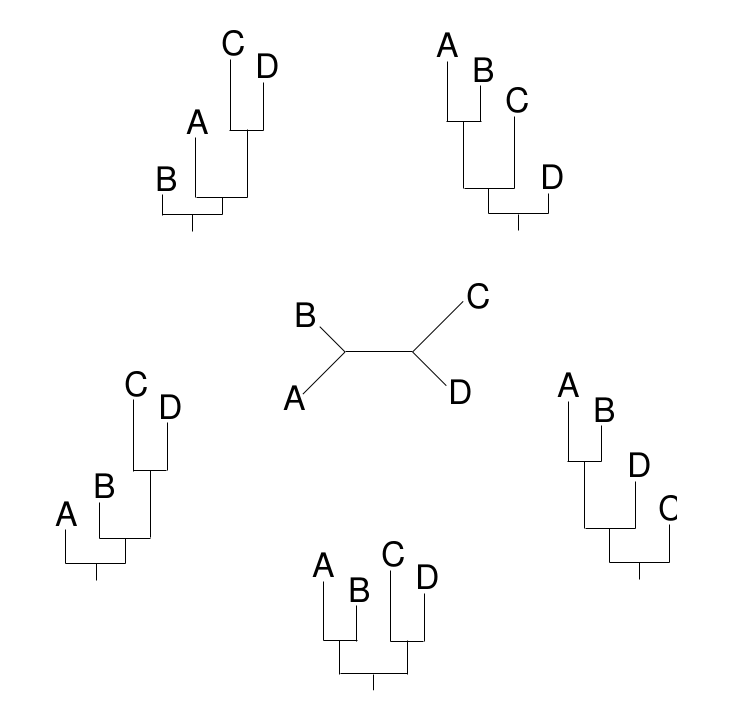
\includegraphics[height=3in]{fig1}
\caption{\textbf{\textsc{Example of unrooted and rooted trees}}.
An unrooted tree of four species (center) with the branch lengths drawn proportional
to their length in terms of expected number of substitutions per site. The five trees 
surrounding the central, unrooted, tree show the five possible rooted trees that result
from the unrooted tree. 
}
\label{fig1}
\end{figure}

The third component of a model of molecular evolution is a process that describes how the characters change on the
phylogeny. All model-based methods of phylogenetic inference, including maximum likelihood and Bayesian estimation
of phylogeny, currently assume that character change occurs according to a continuous-time Markov chain. At the heart
of any continuous-time Markov chain is a matrix of rates, specifying the rate of change from one state to another. For
example, the instantaneous rate of change under the model described by Hasegawa et al. (1984, 1985; hereafter called the HKY85 model) is
\begin{equation*}
{\mathbf Q} = \{q_{ij}\} = \left( \begin{array}{cccc}
-               &  \pi_C & \kappa \pi_G & \pi_T \\
\pi_A & -               & \pi_G & \kappa \pi_T \\
\kappa \pi_A & \pi_C & -               & \pi_T \\
\pi_A & \kappa \pi_C & \pi_G & -               \\
\end{array} \right) \mu
\end{equation*}
This matrix specifies the rate of change from one nucleotide to another; the rows and columns of the matrix are
ordered $A, C, G, T$, so that the rate of change from $C \rightarrow G$ is $q_{CG} = \pi_G$. Similarly, the rates
of change between $C \rightarrow T$, $G \rightarrow A$, and $T \rightarrow C$, are $q_{CT} = \kappa \pi_T$,
$q_{GA} = \kappa \pi_A$, and $q_{TG} = \pi_G$, respectively. 
The diagonals of the rate matrix, denoted with the
dash, are specified such that each row sums to zero. Finally, the rate matrix is rescaled such that the mean rate of
substitution is one. This can be accomplished by setting $\mu = -1 / \sum_{i\in \{A,C,G,T\}} \pi_i q_{ii}$. This rescaling of the rate matrix such that the mean
rate is one allows the branch lengths on the phylogenetic tree to be interpreted as expected number of nucleotide
substitutions per site.

We will make a few important points about the rate matrix. First, the rate matrix may have free parameters. For example,
the HKY85 model has the parameters $\kappa$, $\pi_A$, $\pi_C$, $\pi_G$, and $\pi_T$. 
The parameter $\kappa$ is the transition/transversion rate bias; when $\kappa = 1$ transitions occur at the same rate as transversions.
Typically, the transition/transversion rate ratio, estimated using maximum likelihood or Bayesian inference, is estimated
to be greater then one; transitions occur at a higher rate than transversions.
The other parameters---$\pi_A$, $\pi_C$, $\pi_G$, and $\pi_T$---are the base frequencies, and have a biological interpretation
as the frequency of the different nucleotides and are also, incidentally, the stationary probabilities of the process (more on stationary probabilities
later).
Second, the rate matrix, ${\mathbf Q}$, can be used to calculate
the transition probabilities and the stationary distribution of the substitution process. The transition probabilities and
stationary distribution play a key role in calculating the likelihood, and we will spend more time here developing an intuitive
understanding of these concepts.

\subsubsection{Transition probabilities} Let us consider a specific example of a rate matrix, with all of the parameters of the model taking
specific values. For example, if we use the HKY85 model and fix the parameters to 
$\kappa = 5$, $\pi_A = 0.4$, $\pi_C = 0.3$, $\pi_G = 0.2$, and $\pi_T = 0.1$, we get the following matrix of instantaneous
rates
$$
{\mathbf Q} = \{q_{ij}\} = \left( \begin{array}{rrrr}
-0.886 &  0.190 &  0.633 &  0.063 \\
 0.253 & -0.696 &  0.127 &  0.316 \\
 1.266 &  0.190 & -1.519 &  0.063 \\
 0.253 &  0.949 &  0.127 & -1.329 \\
\end{array} \right)
$$
Note that these numbers are not special in any particular way. That is to say, they are not based upon any observations
from a real data set, but are rather arbitrarily picked to illustrate a point. The point is that one can interpret the rate matrix
in the physical sense of specifying how changes occur on a phylogenetic tree. Consider the very simple case of a single
branch on a phylogenetic tree. Let's assume that the branch is $v=0.5$ in length and that the ancestor of the branch is
the nucleotide $G$. The situation we have is something like that shown in Figure~2A. How can we simulate the evolution
of the site starting from the $G$ at the ancestor? The rate matrix tells us how to do this. First of all, because the current state of the process is $G$,  the only relevant row of the rate matrix is the third one:
$$
{\mathbf Q} = \{q_{ij}\} = \left( \begin{array}{cccc}
\cdot   &   \cdot &    \cdot &  \cdot \\
\cdot   &   \cdot &    \cdot &  \cdot \\
1.266 &  0.190 & -1.519 &  0.063 \\
\cdot   &   \cdot &    \cdot & \cdot \\
\end{array} \right)
$$
The overall rate of change away from nucleotide $G$ is $q_{GA} + q_{GC} + q_{GT} = 1.266 + 0.190 + 0.063 = 1.519$.
Equivalently, the rate of change away from nucleotide $G$ is simply $-q_{GG} = 1.519$. We wait an exponentially
distributed amount of time with rate 1.519 until the next substitution occurs. One can easily construct exponential
random variables from uniform random variables using the equation
\begin{figure}[t]
\centering
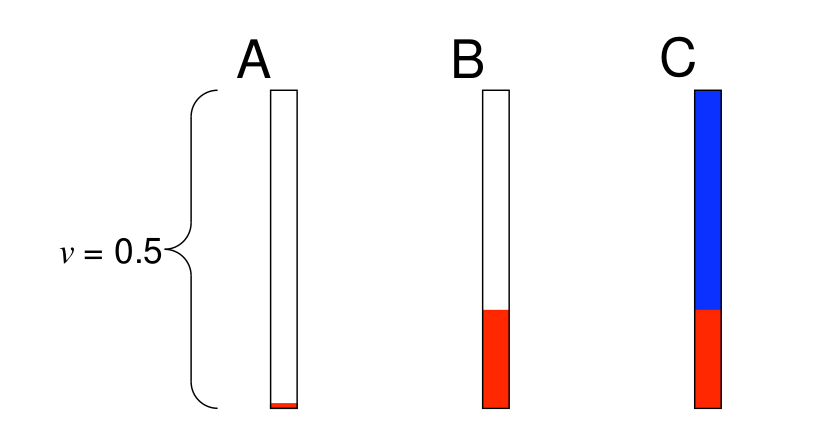
\includegraphics[height=1.75in]{fig2}
\caption{\textbf{\textsc{Simulation under the HKY85 substitution process}}.
A single realization of the substitution process under the HKY85 model when 
$\kappa = 5$, $\pi_A = 0.4$, $\pi_C = 0.3$, $\pi_G = 0.2$, and $\pi_T = 0.1$. The length of the branch
is $v = 0.5$ and the starting nucleotide is $G$ (red). A, The process starts in nucleotide G. B, The first change is 0.152
units up the branch. C, the change is from G to A (blue). The time at which the next change occurs exceeds the total
branch length, so the process ends in state C. }
\label{fig2}
\end{figure}
$$
t = -{1 \over \lambda} \log_e(u)
$$
where $\lambda$ is the rate and $u$ is a uniform(0,1) random number. For example, our calculator has a uniform(0,1) random number generator.
The first number it generated is $u = 0.794$. This means that the next time at which a substitution occurs is
0.152 up from the root of the tree (using $\lambda = 1.519$; Figure~2B). The rate matrix also specifies the probabilities of a change from $G$
to the nucleotides $A$, $C$, and $T$.  These probabilities are
$$
\begin{array}{ccc}
G \rightarrow A: {1.266\over 1.519}=0.833, &  G \rightarrow C: {0.190\over 1.519}=0.125, & G \rightarrow T: {0.063 \over 1.519}=0.042 \\
\end{array} 
$$
To determine what nucleotide the process changes to we would generate another uniform(0,1) random number (again
called $u$). If $u$ is between 0 and 0.833, we will say that we had a change from $G$ to $A$. If the random number
is between 0.833 and 0.958 we will say that we had a change from $G$ to $C$. Finally, if the random number $u$ is
between 0.958 and 1.000, we will say we had a change from $G$ to $T$. The next number generated on our calculator
was $u = 0.102$, which means the change was from $G$ to $A$. The process is now in a different state (the nucleotide
$A$) and the relevant row of the rate matrix is
$$
{\mathbf Q} = \{q_{ij}\} = \left( \begin{array}{cccc}
-0.886 &  0.190 &  0.633 &  0.063 \\
\cdot & \cdot &  \cdot &  \cdot \\
\cdot &  \cdot & \cdot &  \cdot \\
\cdot &  \cdot &  \cdot & \cdot \\
\end{array} \right)
$$
We wait an exponentially distributed amount of time with parameter
$\lambda = 0.886$ until the next substitution occurs. When the substitution occurs, it is to a $C$, $G$, or $T$
with probabilities ${0.190 \over 0.886} = 0.214$, ${0.633 \over 0.886} = 0.714$, and ${0.063 \over 0.886} = 0.072$,
respectively. This process of generating random and exponentially distributed times until the next substitution occurs
and then determining (randomly) what nucleotide the change is to is repeated until the process exceeds the length
of the branch. The state the process is in when it passes the end of the branch is recorded. In the example of Figure~2,
the process started in state $G$ and ended in state $A$. (The next uniform random variable generated on our
calculator was $u = 0.371$, which means that the next substitution would occur 1.119 units above the substitution
from $G \rightarrow A$. The process is in the state $A$ when it passed the end of the branch.)
The only non-random part of the entire procedure was the initial
decision to start the process in state $G$. All other aspects of the simulation used a uniform random number generator
and our knowledge of the rate matrix to simulate a single realization of the HKY85 process of DNA substitution. 

\begin{figure}[t]
\centering
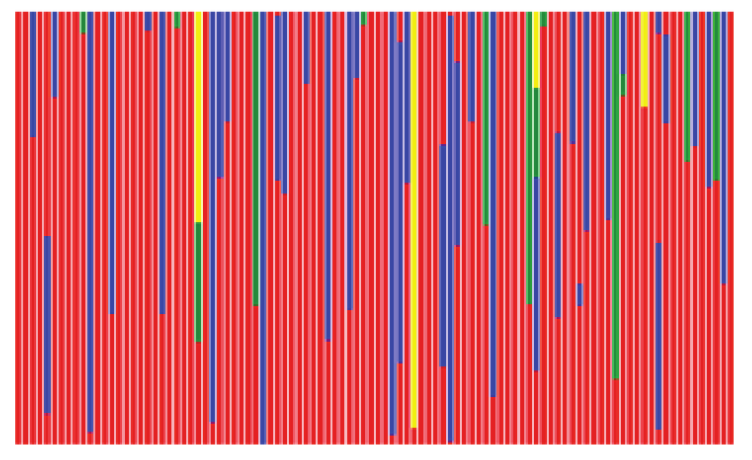
\includegraphics[height=2in]{fig3}
\caption{\textbf{\textsc{Simulations under the HKY85 substitution process}}.
One hundred simulations under the HKY85 model when 
$\kappa = 5$, $\pi_A = 0.4$, $\pi_C = 0.3$, $\pi_G = 0.2$, and $\pi_T = 0.1$. The length of the branch
is $v = 0.5$ and the starting nucleotide is always $G$. Blue, A; green, C; red: G; yellow, T. 
}
\label{fig3}
\end{figure}

This Monte Carlo procedure for simulating the HKY85 process of DNA substitution can be repeated. Figure~3 shows
100 realizations of the HKY85 substitution process where each simulation started with the nucleotide $G$. 
The following table summarizes the results of the
100 simulations:
\begin{center}
\begin{tabular}{ccc}
Starting & Ending & Number of \\
Nucleotide & Nucleotide &  Replicates \\ \hline
G & A & 27 \\
G & C & 10 \\
G & G & 59 \\
G & T & 4 \\
\end{tabular}
\end{center}
This table can be interpreted as a Monte Carlo approximation of the {\it transition probabilities} from nucleotide
$G$ to nucleotide $i \in (A,C,G,T)$. Specifically, the Monte Carlo approximations are 
$p_{GA}(0.5) \approx 0.27$, 
$p_{GC}(0.5) \approx 0.10$, 
$p_{GG}(0.5) \approx 0.59$, and
$p_{GT}(0.5) \approx 0.04$.
These approximate probabilities are all conditioned on the starting nucleotide being $G$ and the branch length
being $v = 0.5$. Figure~4 shows simulations
when the starting nucleotide is $A$, $C$, $G$, or $T$ (the branch length remains $v=0.5$). The simulations allow us to fill out the following table with the approximate
transition probabilities:
\begin{center}
\begin{tabular}{crcccc}
&    & \multicolumn{4}{c}{Ending} \\
&    & \multicolumn{4}{c}{Nucleotide} \\
                     &    & A  & C & G & T \\ \cline{2-6}
                     & A \vline & 0.67 & 0.13 & 0.20 & 0.00 \\
Starting       & C \vline & 0.13 & 0.70 & 0.07 & 0.10 \\
Nucleotide & G \vline & 0.27 & 0.10 & 0.59 & 0.04 \\
                     & T \vline & 0.12 & 0.30 & 0.08 & 0.50 \\ \cline{2-6}
\end{tabular}
\end{center}
Clearly, these numbers are only crude approximations to the true transition probabilities; after all, each row in the table is based on only 100 
Monte Carlo simulations. However, they do illustrate the meaning
of the transition probabilities; the transition probability, $p_{ij}(v)$, is the probability that the substitution process ends in nucleotide
$j$ conditioned on it starting in nucleotide $i$ after an evolutionary amount of time $v$. The table of approximate transition probabilities,
above, can be interpreted as a matrix of probabilities, usually denoted ${\mathbf P}(v)$. 
Fortunately, we do not need to rely on Monte Carlo simulation to approximate the transition probability matrix. Instead, we can
calculate the transition probability matrix exactly using matrix exponentiation:
$$
{\mathbf P}(v) = e^{{\mathbf Q} v}
$$
For the case we have been simulating, the exact transition probabilities (to four decimal places) are
$$
{\mathbf P}(0.5) = \{p_{ij}(0.5)\} = \left( \begin{array}{rrrr}
0.7079 & 0.0813 & 0.1835 & 0.0271 \\
0.1085 & 0.7377 & 0.0542 & 0.0995 \\
0.3670 & 0.0813 & 0.5244 & 0.0271 \\
0.1085 & 0.2985 & 0.0542 & 0.5387 \\
\end{array} \right)
$$
The transition probability matrix accounts for all the possible ways the process could end up in nucleotide
$j$ after starting in nucleotide $i$. In fact, each of the infinite possibilities is weighted by its probability
under the substitution model.

\begin{figure}[t]
\centering
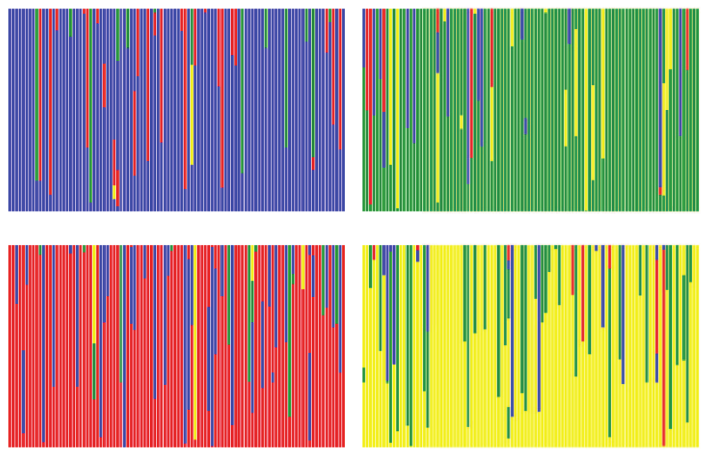
\includegraphics[height=2in]{fig4}
\caption{\textbf{\textsc{Simulations under the HKY85 substitution process}}.
One hundred simulations under the HKY85 model when 
$\kappa = 5$, $\pi_A = 0.4$, $\pi_C = 0.3$, $\pi_G = 0.2$, and $\pi_T = 0.1$. The starting nucleotide is
A, C, G, or T for the upper left, upper right, lower left and lower right panels, respectively. The length of the branch
is $v = 0.5$. Blue, A; green, C; red: G; yellow, T. 
}
\label{fig4}
\end{figure}

\subsubsection{Stationary distribution} The transition probabilities provide the probability of ending in a particular nucleotide after
some specific amount of time (or opportunity for substitution, $v$). These transition probabilities are conditioned
on starting in a particular nucleotide. What do the transition probability matrices look like as $v$ increases? The following
transition probability matrices show the effect of increasing branch length:
$$
\begin{array}{cc}
{{\mathbf P}(0.00) = \left( \begin{array}{rrrr}
1.000 & 0.000 & 0.000 & 0.000 \\
0.000 & 1.000 & 0.000 & 0.000 \\
0.000 & 0.000 & 1.000 & 0.000 \\
0.000 & 0.000 & 0.000 & 1.000 \\
\end{array} \right)}
 &
{{\mathbf P}(0.01) = \left( \begin{array}{rrrr}
0.991 & 0.002 & 0.006 & 0.001 \\
0.003 & 0.993 & 0.001 & 0.003 \\
0.013 & 0.002 & 0.985 & 0.001 \\
0.003 & 0.009 & 0.001 & 0.987 \\
\end{array} \right)}
\end{array}
$$
$$
\begin{array}{cc}
{{\mathbf P}(0.10) = \left( \begin{array}{rrrr}
0.919 & 0.018 & 0.056 & 0.006 \\
0.024 & 0.934 & 0.012 & 0.029 \\
0.113 & 0.018 & 0.863 & 0.006 \\
0.025 & 0.086 & 0.012 & 0.877 \\
\end{array} \right)}
 &
{{\mathbf P}(0.50) = \left( \begin{array}{rrrr}
0.708 & 0.081 & 0.184 & 0.027 \\
0.106 & 0.738 & 0.054 & 0.100 \\
0.367 & 0.081 & 0.524 & 0.027 \\
0.109 & 0.299 & 0.054 & 0.539 \\
\end{array} \right)}
\end{array}
$$
$$
\begin{array}{cc}
{{\mathbf P}(1.00) = \left( \begin{array}{rrrr}
0.580 & 0.141 & 0.232 & 0.047 \\
0.188 & 0.587 & 0.094 & 0.131 \\
0.464 & 0.141 & 0.348 & 0.047 \\
0.188 & 0.394 & 0.094 & 0.324 \\
\end{array} \right)}
 &
{{\mathbf P}(5.00) = \left( \begin{array}{rrrr}
0.411 & 0.287 & 0.206 & 0.096 \\
0.383 & 0.319 & 0.192 & 0.106 \\
0.411 & 0.287 & 0.206 & 0.096 \\
0.383 & 0.319 & 0.192 & 0.107 \\
\end{array} \right)}
\end{array}
$$
$$
\begin{array}{cc}
{{\mathbf P}(10.0) = \left( \begin{array}{rrrr}
0.401 & 0.299 & 0.200 & 0.099 \\
0.399 & 0.301 & 0.199 & 0.100 \\
0.401 & 0.299 & 0.200 & 0.099 \\
0.399 & 0.301 & 0.199 & 0.100 \\
\end{array} \right)}
 &
{{\mathbf P}(100) = \left( \begin{array}{rrrr}
0.400 & 0.300 & 0.200 & 0.100 \\
0.400 & 0.300 & 0.200 & 0.100 \\
0.400 & 0.300 & 0.200 & 0.100 \\
0.400 & 0.300 & 0.200 & 0.100 \\
\end{array} \right)}
\\
\end{array}
$$
(Each matrix was calculated under the HKY85 model with 
$\kappa = 5$, $\pi_A = 0.4$, $\pi_C = 0.3$, $\pi_G = 0.2$, and $\pi_T = 0.1$.)
Note that as the length of a branch, $v$, increases, the probability of ending up in a particular nucleotide converges
to a single number, regardless of the starting state. For example, the probability of ending up in $C$ is about 0.300
when the branch length is $v=100$. This is true regardless of whether the process starts in $A$, $C$, $G$, or $T$.
The substitution process has in a sense `forgotten' its starting state.

The stationary distribution is the probability of observing a particular state when the branch length increases without limit
($v \rightarrow \infty$). The stationary probabilities of the four nucleotides are $\pi_A = 0.4$, $\pi_C = 0.3$, $\pi_G = 0.2$,
and $\pi_T = 0.1$ for the example discussed above. The models typically used in phylogenetic analyses have the stationary
probabilities built into the rate matrix, ${\mathbf Q}$. You will notice that the rate matrix for the HKY85
model has parameters $\pi_A$, $\pi_C$, $\pi_G$, and $\pi_T$, and that the stationary frequencies of the four nucleotides
for our example match the input values for our simulations. Building the stationary frequency of the process into the
rate matrix, while somewhat unusual, makes calculating the likelihood function easier. For one, specifying the stationary
distribution saves the time of figuring out what the stationary distribution is (which involves solving the equation
$\pi {\mathbf Q} = {\mathbf 0}$). For another, it allows one to more easily specify  a time reversible substitution model.
[A time reversible substitution model has the property that $\pi_i q_{ij} = \pi_j q_{ji}$ for all $i, j \in (A,C,G,T)$, $i \neq j$.]
Practically speaking, time reversibility means that we can work with unrooted trees instead of rooted trees.

\subsubsection{Calculating the likelihood} The transition probabilities and stationary distribution are used when calculating
the likelihood. For example, consider the following alignment of sequences for five species\footnote{This alignment was simulated on the tree of Figure~5 under the HKY85 model of DNA substitution. Parameter values for
the simulation can be found in the caption of Table~1.}:
\begin{verbatim}
Species 1   TAACTGTAAAGGACAACACTAGCAGGCCAGACGCACACGCACAGCGCACC
Species 2   TGACTTTAAAGGACGACCCTACCAGGGCGGACACAAACGGACAGCGCAGC
Species 3   CAAGTTTAGAAAACGGCACCAACACAACAGACGTATGCAACTGACGCACC
Species 4   CGAGTTCAGAAGACGGCACCAACACAGCGGACGTATGCAGACGACGCACC
Species 5   TGCCCTTAGGAGGCGGCACTAACACCGCGGACGAGTGCGGACAACGTACC
\end{verbatim}
This is clearly a rather small alignment of sequences to use for estimating phylogeny, but it will illustrate
how likelihoods are calculated. The likelihood is the probability of the alignment of sequences, conditioned on a tree
with branch lengths. The basic procedure is to calculate the probability of each site (column) in the matrix. Assuming that
the substitutions are independent across sites, the probability of the entire alignment is simply the product of the probabilities
of the individual sites. 

\begin{figure}[t]
\centering
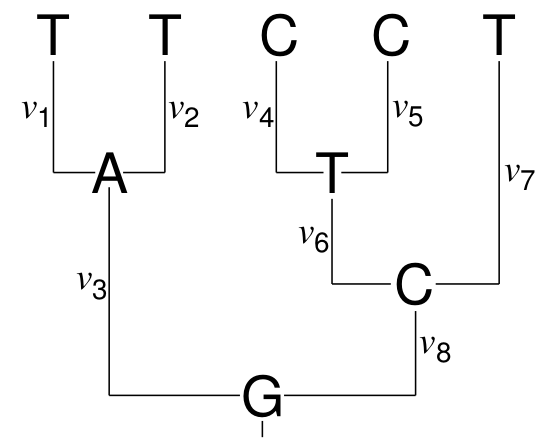
\includegraphics[height=2in]{fig5}
\caption{\textbf{\textsc{A tree with states assigned to the tips}}.
One of the possible (rooted) trees describing the evolutionary history of the five species. The states at the first
site in the alignment of the text are shown at the tips of the tree. The states at the interior nodes of the tree are also
shown, though in reality these states are not observed. The length of the $i$th branch is denoted $v_i$. }
\label{fig5}
\end{figure}

How is the likelihood at a single site calculated? Figure~5 shows the observations at the first site ($T$, $T$, $C$, $C$, and $T$)
at the tips of one of the possible phylogenetic trees for five species. The tree in Figure~5 is unusual in that we will
assume that the nucleotide states at the interior nodes of the tree are also known. This is clearly a bad assumption, because
we cannot directly observe the nucleotides that occurred at any point on the tree in the distant past. For now, however, ignore
this fact and bear with us. The probability of observing the configuration of nucleotides at the tips and interior nodes of
the tree in Figure~5 is
\begin{eqnarray*}
\lefteqn{\Pr(TTCCT , ATCG | \tau, {\mathbf v}, \theta ) =} \\
& & \pi_G \,
p_{GA}(v_3) \,
p_{AT}(v_1) \,
p_{AT}(v_2) \,
p_{GC}(v_8) \,
p_{CT}(v_6) \,
p_{CT}(v_7) \,
p_{TC}(v_4) \,
p_{TC}(v_5)
\end{eqnarray*}
Here we show the probability of the observations (TTCCT) and the states at the interior nodes of the tree (ATCG)
conditioned on the tree ($\tau$), branch lengths (${\mathbf v}$), and other model parameters  ($\theta$).
Note that to calculate the probability of the states at the tips of the tree, we used the stationary probability
of the process ($\pi$) and also the transition probabilities [$p_{ij}(v)$]. The stationary probability of the substitution
process was used to calculate the probability of the nucleotide at the root of the tree. In this case, we are assuming that
the substitution process has been running a very long time before it reached the root of our five species tree. We then use
the transition probabilities to calculate the probabilities of observing the states at each end of the branches. When taking
the product of the transition probabilities, we are making the additional assumption that the substitutions on each branch
of the tree are independent of one another. This is probably a reasonable assumption for real data sets.

The probability of observing the states at the tips of the tree, described above, was conditioned on the interior nodes
of the tree taking specific values (in this case $ATCG$). To calculate the unconditional probability of the observed states
at the tips of the tree, we sum over all possible combinations of nucleotide states that can be assigned to the interior nodes
of the tree
$$
\Pr(TTCCT | \tau, {\mathbf v}, \theta ) = \sum_{w} \sum_{x} \sum_{y} \sum_{z} 
\Pr(TTCCT , w x y z | \tau, {\mathbf v}, \theta )
$$
where $w,x,y,z \in  (A,C,G,T)$. Averaging the probabilities over all combinations of states at the interior nodes of the
tree accomplishes two things. First, we remove the assumption that the states at the interior nodes take specific
values. Second, because the transition probabilities account for all of the possible ways we could have state $i$ at
one end of a branch and state $j$ at the other, the probability of the site is also averaged over all possible character
histories. Here, we think of a character history as one realization of changes on the tree that is consistent with the
observations at the tips of the tree. For example, the parsimony method, besides calculating the minimum number of
changes on the tree, also provides a character history; the character history favored by parsimony is the one that minimizes the number of changes
required to explain the data. In the case of likelihood-based methods, the likelihood accounts for all possible character histories,
with each history weighted by its probability under the substitution model. Nielsen ([ref]) described a method for sampling
character histories in proportion to their probability that relies on the interpretation of the rate matrix as specifying waiting
times between substitutions. His method provides a means to reconstruct the history of a character
that does not inherit the flaws of the parsimony method. Namely, Nielsen's method allows multiple changes on a single
branch and also allows for non-parsimonious reconstructions of a character's history.

\begin{table}[b]
\centering
\caption{\textbf{\textsc{Probabilities of individual sites}}.
The probabilities of the fifty sites for the example alignment from the text. The likelihoods are calculated assuming the tree
of Figure~5 with the branch lengths being $v_1 = 0.1$, $v_2 = 0.1$, $v_3 = 0.2$, $v_4 = 0.1$, $v_5 = 0.1$, $v_6 = 0.1$,
$v_7 = 0.2$, and $v_8 = 0.1$. The substitution model parameters were also fixed, with 
$\kappa = 5$, $\pi_A = 0.4$, $\pi_C = 0.3$, $\pi_G = 0.2$, and $\pi_T = 0.1$.}
\begin{tabular}{cccccccccc}
Site  & Prob.               & Site        & Prob.               & Site        & Prob.              & Site        & Prob.               & Site        & Prob.              \\ \hline
1	&	0.004025	&	11	&	0.029483	&	21	&	0.179392	&	31	&	0.179392	&	41	&	0.003755 \\
2	&	0.001171	&	12	&	0.006853	&	22	&	0.001003	&	32	&	0.154924	&	42	&	0.005373 \\
3	&	0.008008	&	13	&	0.024885	&	23	&	0.154924	&	33	&	0.007647	&	43	&	0.016449 \\
4	&	0.002041	&	14	&	0.154924	&	24	&	0.179392	&	34	&	0.000936	&	44	&	0.029483 \\
5	&	0.005885	&	15	&	0.007647	&	25	&	0.005719	&	35	&	0.024885	&	45	&	0.154924 \\
6	&	0.000397	&	16	&	0.024124	&	26	&	0.001676	&	36	&	0.000403	&	46	&	0.047678 \\
7	&	0.002802	&	17	&	0.154924	&	27	&	0.000161	&	37	&	0.024124	&	47	&	0.010442 \\
8	&	0.179392	&	18	&	0.004000	&	28	&	0.154924	&	38	&	0.154924	&	48	&	0.179392 \\
9	&	0.024124	&	19	&	0.154924	&	29	&	0.001171	&	39	&	0.011088	&	49	&	0.002186 \\
10	&	0.024885	&	20	&	0.004025	&	30	&	0.047678	&	40	&	0.000161	&	50	&	0.154924 \\ \hline
\end{tabular}
\label{tab1}
\end{table}

Before moving on to some applications of Bayesian estimation in molecular evolution, we will make two final points. First,
in practice no computer program actually evaluates all combinations of nucleotides that can be assigned to
the interior nodes of a tree when calculating the probability of observing the data at a site. There are simply too many combinations
for trees of even small size. For example, for a tree of 100 species, there are 99 interior nodes and $4.02 \times 10^{59}$ combinations
of nucleotides at the ancestral nodes on the tree. 
Instead, Felsenstein's (1981)
pruning algorithm is used to calculate the likelihood at a site. Felsenstein's method is mathematically equivalent to the
summation shown above, but can evaluate the likelihood at a site in a fraction of the time it would take to plow through all combinations of ancestral states. Second, the overall likelihood of
a character matrix is the product of the site likelihoods. If we assume that the tree of Figure~5 is correct
(with all of the parameters taking the values specified in the caption of Table~1), then the probability of observing the data
is
$$
0.004025 \times 0.001171 \times 0.008008 \times \ldots \times  0.154924 = 1.2316 \times 10^{-94}
$$
where there are fifty factors, each factor representing the probability of an individual site (column) in the alignment. Table~1 shows
the probabilities of all fifty sites for the tree of Figure~5. Note that the overall probability of observing the data is a very small
number ($\approx 10^{-94}$). This is typical of phylogenetic problems and results from the simple fact that many numbers between
0 and 1 are multiplied together. Computers cannot accurately hold very small numbers in memory. Programmers avoid this problem
of computer ``underflow'' by using the log probability of observing the data. The log probability of observing the sample alignment of
sequences presented earlier is  $\log_e \ell = \log_e(1.2316 \times 10^{-94}) = -216.234734$. The log likelihood can be accurately
stored in computer memory.

\subsection{Phylogeny estimation}

\subsubsection{Frequentist and Bayesian perspectives on phylogeny estimation}

The phylogenetic model described in the preceding section has numerous parameters. Minimally, the parameters include the
topology of the tree and the lengths of the branches on the tree. In the following, we imagine that every possible tree is labelled: 
$\tau_1, \tau_2, \ldots, \tau_{B(n)}$. Each tree has its own set of branches, and each branch has a length in terms of expected number of
substitutions per site. The lengths of the branches on the $i$th tree are denoted ${\mathbf v}_i = (v_1, v_2, \ldots, v_{2n-3})$. In addition,
there may be parameters associated with the substitution model. 
The parameters of the substitution model will be denoted ${\mathbf \theta}$. 
For the HKY85 model the parameters are ${\mathbf \theta} = (\kappa, \pi_A, \pi_C, \pi_G, \pi_T)$, but other substitution models may
have more or fewer parameters than the HKY85 model. 
When all of the parameters are specified, one can calculate the likelihood function using the general ideas described in the previous
section. The likelihood will be denoted $\ell(\tau_i, {\mathbf v}_i, {\mathbf \theta})$ and is proportional to the probability of observing the
data conditioned on the model parameters taking specific values 
($\ell(\tau_i, {\mathbf v}_i, {\mathbf \theta}) \propto \Pr[ {\mathbf X} |  \tau_i, {\mathbf v}_i, {\mathbf \theta} ] $; the alignment of
sequences is ${\mathbf X}$).

Which of the possible trees best explains the alignment of DNA sequences? This is among the most basic questions asked in many molecular evolution studies. In a maximum likelihood analysis the answer is straight forward: the
best estimate of phylogeny is the tree that maximizes the likelihood. This is equivalent to finding the tree that makes the observations
most probable. For the toy alignment of sequences given in the previous section, the likelihood is maximized when the tree of
Figure~5 is used. The other 14 possible trees had a lower likelihood. (This is not surprising because the sequences were simulated on the tree of Figure~5.)
How was the maximum likelihood tree found? In this case, the program
PAUP* (Swofford, 2002) visited each of the 15 possible trees. For each tree, it found the combination of parameters that maximized the
likelihood. In this analysis, we assumed the HKY85 model, so the parameters included the transition/transversion
rate ratio and the nucleotide frequencies. After maximizing the likelihood for each tree, the program picked that tree with the largest likelihood as the best estimate of phylogeny. The approach was described earlier in this chapter; the nuisance parameters (here all of the parameters
except for the topology of the tree) are dealt with by maximizing the likelihood with respect to them. The tree of Figure~5 has a maximum
likelihood score of $-211.25187$. The parameter estimates on this tree are:
$\hat{v}_1 = 0.182$,
$\hat{v}_2 = 0.124$,
$\hat{v}_{3 + 8} = 0.226$,
$\hat{v}_4 = 0.162$,
$\hat{v}_5 = 0.018$,
$\hat{v}_6 = 0.159$,
$\hat{v}_7 = 0.199$,
$\hat{\kappa} = 5.73$,
$\hat{\pi}_A = 0.329$,
$\hat{\pi}_C = 0.329$,
$\hat{\pi}_G = 0.253$, and
$\hat{\pi}_T = 0.089$.
The method of maximum likelihood and the program PAUP*, often used to find maximum likelihood trees, are described in more
detail in Chapter [NUMBER]. Importantly, there are many computational shortcuts that can be taken to speed up calculation of the maximum likelihood
tree.

In a Bayesian analysis, inferences are based upon the posterior probability distribution of the parameters. The joint posterior
probability of all the parameters  is calculated using Bayes's theorem as
$$
\Pr[\tau_i, {\mathbf v}_i, {\mathbf \theta} | {\mathbf X}] = 
{\Pr[ {\mathbf X} |  \tau_i, {\mathbf v}_i, {\mathbf \theta} ] \times \Pr[\tau_i, {\mathbf v}_i, {\mathbf \theta}]
 \over 
\Pr[ {\mathbf X}] }
$$
The posterior probability is equal to the likelihood ($\Pr[ {\mathbf X} |  \tau_i, {\mathbf v}_i, {\mathbf \theta} ]$) times the prior probability of the parameters ($\Pr[\tau_i, {\mathbf v}_i, {\mathbf \theta}]$) divided by a normalizing constant
($\Pr[ {\mathbf X}]$). The normalizing constant involves a summation over all possible trees and, for each tree, integration over all possible
combinations of branch lengths and parameter values. Clearly, the Bayesian method is similar to the method of maximum likelihood; after
all, both methods make the same assumptions about the evolutionary process and use the same likelihood function. However, the Bayesian
method treats all of the parameters as random variables (note that the posterior probability is the probability of the parameters) and the
method also incorporates any prior information the biologist might have about the parameters through the prior probability distribution of
the parameters.  

Unfortunately, one cannot calculate the posterior probability distribution of trees analytically. Instead, one resorts to a heuristic algorithm to
approximate posterior probabilities of trees. The program MrBayes (Huelsenbeck and Ronquist, [year]; Ronquist and Huelsenbeck, [year]) 
uses Markov chain Monte Carlo (MCMC) to approximate posterior probabilities
of phylogenetic trees (and the posterior probability density of the model parameters). Briefly, a Markov chain is constructed that has as its
state space the parameter values of the model and a stationary distribution that is the posterior probability of the parameters. Samples drawn
from this Markov chain while at stationarity are valid, albeit dependent, samples from the posterior probability distribution of the parameters. If
one is interested in the posterior probability of a particular phylogenetic tree, one simply notes the fraction of the time the Markov chain visited
that tree; the proportion of the time the chain visits the tree is an approximation of that tree's posterior probability. A thorough discussion of MCMC
is beyond the scope of this chapter. However, an excellent description of MCMC and its applications in molecular evolution can be found in
Chapter [NUMBER] (Larget, [YEAR]).

\begin{table}[b]
\centering
\caption{\textbf{\textsc{Summary statistics for the marginal posterior probability density distributions of the substitution parameters}}.
The mean, median, variance, and 95\% credible interval of the marginal posterior probability density distribution of the substitution
parameters of the HKY85 model. The parameters are discussed in the text.}
\begin{tabular}{cccccc}
                    &             &                  & \multicolumn{2}{c}{95\% Cred. Interval} & \\ \cline{4-5}
Parameter & Mean & Variance & Lower & Upper & Median \\ \hline
$V$           &  0.990  &  0.025  &  0.711   & 1.333  &  0.980   \\
$\kappa$ &  5.576  &  4.326 &  2.611 &  10.635  &  5.219   \\
$\pi_A$    &  0.323  &  0.002  &  0.235  &  0.418  &  0.323   \\
$\pi_C$    &  0.331  &  0.002  &  0.238  &  0.433 &  0.329   \\
$\pi_G$    &  0.252  &  0.002  &  0.176  &  0.340 &   0.250   \\
$\pi_T$     &  0.092  &  0.001 &   0.047  &  0.152 &  0.090   \\ \hline
\end{tabular}
\label{tab2}
\end{table}

We performed a Bayesian analysis on the simulated data set discussed above under the HKY85 model. (We describe how to do the Bayesian
analyses performed in this chapter in the second appendix.) 
This is a rather ideal situation because
the example data were simulated on the tree of Figure~5 under the HKY85 model; the model assumed in the Bayesian analysis is not misspecified.
We ran a Markov chain for 1,000,000 cycles using the program MrBayes. The Markov chain visited the tree shown in Figure~5 about 99\% of the
time; the MCMC approximation of the posterior probability of the tree in Figure~5, then, is about 0.99. This can be considered strong evidence in
favor of that tree. The posterior probabilities of phylogenetic trees was calculated by integrating over uncertainty in the other model parameters (such
as branch lengths, the transition/tranversion rate ratio, and base frequencies). However, we can turn the study around and ask questions about the
parameters of the substitution model. Table~2 shows information on the posterior probability density distribution of the substitution model parameters.
The table shows the mean, median, and variance of the marginal posterior probability distribution for the tree length ($V$), transition/transversion
rate ratio ($\kappa$), and base frequencies ($\pi_A$, $\pi_C$, $\pi_G$, $\pi_T$). The table also shows the upper and lower limits of an interval that
contains 95\% of the posterior probability for each parameter. The table shows, for example, that with probability 0.95 the transition/transversion
rate ratio is in the interval (2.611, 10.635). In reality, the transition/transversion rate ratio was in that interval (the data matrix was simulated with
$\kappa = 5$). The mean of the posterior probability distribution for $\kappa$ was 5.576 (which is fairly close to the true value). The interval we constructed
that contains the true value of the parameter with 0.95 probability is called a 95\% credible interval. One can construct a credible set of trees in a similar
manner; simply order the trees from highest to lowest posterior probability, and put the trees into a set (starting from the tree with highest probability)
until the cumulative probability of trees in the set is 0.95. 

One of the great strengths of the Bayesian approach is the ease with which the results of an analysis can be summarized and interpreted. The posterior
probability of a tree has a very simple and direct interpretation: the posterior probability of a tree is the probability that the tree is correct, assuming that
the substitution model is correct. 
It is worth considering how uncertainty in parameter estimates is evaluated in a more traditional phylogenetic approach. Because the tree is not considered
a random quantity in other types of analyses, such as a maximum likelihood phylogenetic analysis, one cannot directly assign a probability to the tree.
Instead one has to resort to a rather complicated thought experiment. The thought experiment goes something like this. Assuming that the phylogenetic
model is correct and that the parameter estimates take the maximum likelihood values (or better yet, their true values), what would the parameter estimates look like on simulated data sets
of the same size as the original data matrix? The distribution of parameter estimates that would be generated in such a study represent the sampling
distribution of the parameter. One could construct an interval from the sampling distribution that contains 95\% of the parameter estimates from the simulated replicates, and this
would be called a confidence interval. A 95\% confidence interval is a random interval containing the true value of the parameter with probability
0.95. Very few people have constructed confidence intervals/sets of phylogenetic trees using simulation. The simulation approach we just described
is referred to as the parametric bootstrap. 
A related approach, called the nonparametric bootstrap, generates data matrices of the same size as the original by randomly sampling columns (sites) of the original data matrix with replacement. Each matrix generated using the bootstrap procedure is then analyzed using maximum likelihood under the same model as
in the original analysis. The nonparametric bootstrap is widely used in phylogenetic analysis.

\subsubsection{Interpreting posterior probabilities on trees}

One of the concerns in Bayesian phylogenetic analysis is the interpretation of the posterior probabilities on trees, or the probabilities of individual clades on
trees. The posterior probabilities are usually compared to the nonparametric bootstrap proportions, and many have expressed the concern that the posterior
probabilities on clades are too high, or that the posterior probabilities do not have an easy interpretation. We find this concern somewhat frustrating, mostly because
the implicit assumption is that the nonparametric bootstrap proportions are in some way the correct number that should be assigned to a tree, and that any
method that gives a different number is in some way suspect. However, it is not clear that the nonparametric bootstrap values on phylogenetic trees should
be the gold standard. Indeed, it has been known for at least a decade now that the interpretation of nonparametric bootstrap values on phylogenetic trees
is problematic, for a variety of reasons summarized in [REFS]. 

\begin{figure}[t]
\centering
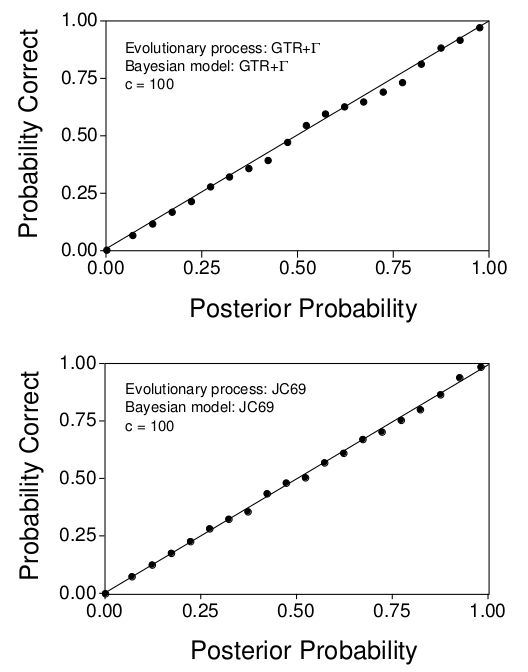
\includegraphics[height=3in]{fig6}
\caption{\textbf{\textsc{The meaning of posterior probabilities under the model}}.
The relationship between the posterior probability of a phylogenetic tree and the probability that the tree is correct when all of the assumptions of
the analysis are satisfied. }
\label{fig6}
\end{figure}

What does the  posterior probability of a phylogenetic tree represent?
Huelsenbeck and Rannala (In Press) performed a small simulation study that did two things. First, it pointed out that the technique many people used to
evaluate the meaning of posterior probabilities was incorrect if the intention was to investigate the best-case scenario for the method (i.e., the situation in
which the Bayesian method does not misspecify the model). Second, it pointed out that the common interpretation of the posterior probability of a phylogenetic
tree is correct; the posterior probability of a phylogenetic tree is the probability that the tree is correct. The catch is that this is true only when the assumptions of the
analysis are correct. Figure~6 summarizes the salient points of the Huelsenbeck and Rannala (In Press) study. The experimental design was as follows. They first
randomly sampled a tree, branch lengths, and substitution model parameters from the prior probability distribution of the parameters. (The tree was a small one, with only
six species.) This is the main difference
between their analysis and all others; they treated the prior model seriously, and generated samples from it instead of considering the parameters of the model fixed
when doing the simulations. For each sample from the prior they simulated a data matrix of 100 sites. They then analyzed the simulated data matrix under the correct
analysis. Figure~6 summarizes the results of 10,000 such simulations for each panel. They simulated data under a very simple model (the JC69 model in which
the base frequencies are all equal and the rates of substitution between states are the same) and a complicated model (the GTR+$\Gamma$ model in which the nucleotide frequencies are free to vary, the rates of substitution between states are allowed to differ, and the rates across sites are gamma distributed). In both
cases, the relationship between posterior probabilities and the probability that the tree is correct is linear; the posterior probability of a tree is the probability that
the tree is correct, at least when the assumptions of the phylogenetic analysis are satisfied. Importantly, to our knowledge posterior probabilities are the only measure
of support that have this simple interpretation.

\begin{figure}[t]
\centering
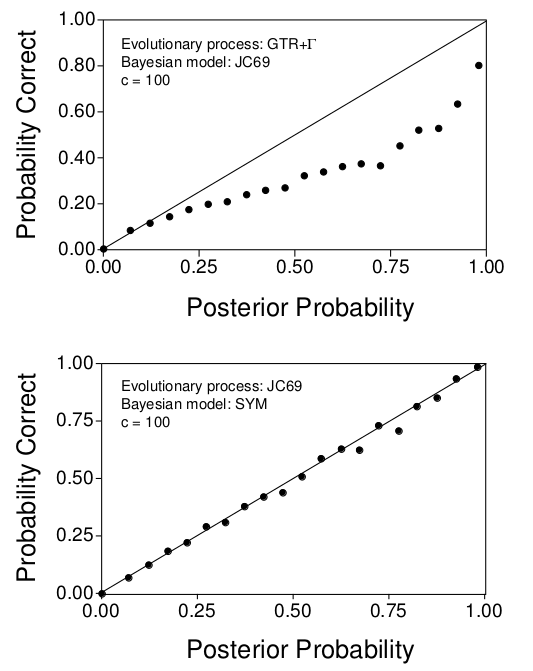
\includegraphics[height=3in]{fig7}
\caption{\textbf{\textsc{The meaning of posterior probabilities when the model is incorrect}}.
The relationship between the posterior probability of a phylogenetic tree and the probability that the tree is correct when all of the assumptions of
the analysis are not met. }
\label{fig7}
\end{figure}

Of course, to some extent the simulation results shown in Figure~6 are superfluous; the posterior probabilities have always been known to have this interpretation, and
the simulations merely confirm the analytical expectation (and incidentally are additional evidence that the program MrBayes is generating valid draws from
the posterior probability distribution of trees, at least for simple problems). The more interesting case is when the assumptions of the analysis are incorrect. 
Suzuki and Nei ([YEAR]) attempted to do such an analysis. Unfortunately, they violated the assumptions of the analysis in a very peculiar way; they simulated data
sets when the underlying phylogeny differed from one gene region to another. This scenario is not a universal concern in phylogenetic analysis (though it
can be a problem in the analysis of closely related species, in bacterial phylogenetics, or in population studies). The common worry is that the substitution model
is incorrect. Huelsenbeck and Rannala (In Press) performed a few simulations when the assumptions of the analysis are incorrect (Figure~7).
The top panel in Figure~7 shows the case when the evolutionary model is not incorporating some important parameters (the model is under-specified). In this
case the relationship between posterior probabilities and the probability that the tree is correct is not linear. Instead, the method places too much posterior probability
on incorrect trees. The situation is not so dire when the evolutionary model has unnecessary parameters (bottom panel in Figure~7).

\subsubsection{Bayesian model choice}

It appears that Bayesian analysis can be sensitive to model misspecification. It is important to note that the best tree selected under the Bayesian criterion is unlikely
to differ significantly from the maximum likelihood tree, mostly because the prior should have a small effect on phylogeny choice when the data set is reasonably
large. It is also important to note that it is not really a problem with the Bayesian method, but rather with the models used to analyze the data. In a sense, biologists
have a method in hand that, in principle, has some very desirable properties: it is fast, allows analysis of complex models in a timely way, and has a correct
and simple interpretation, when the assumptions of the analysis are satisfied. 

The simulation studies summarized in the previous section, along with scores of simulation studies that examine the performance of phylogenetic methods
(see [REFS]), suggest that it
is important to analyze sequence data under as realistic a model as possible. Unfortunately, even the most complicated models currently used in phylogenetic analysis 
are quite simple and fail to capture important evolutionary processes that generated the sequence data. Phylogenetic models need to be improved to
capture evolutionary processes most likely to influence phylogeny estimation. It is impossible to know with certainty what advances will be made in improving
phylogenetic models, but we can speculate on what the future might hold. For one, it seems important to
relax the assumption that the substitution process in homogeneous over the entire phylogenetic history of the organisms under study. This assumption might
be relaxed in a number of ways. For example, Foster ([YEAR]) has relaxed the assumption that nucleotide frequencies are constant over time and [PEOPLE]
([YEAR]) relaxed the assumption that the GC content is a constant over a phylogenetic tree. Other such improvements are undoubtedly in store, and Bayesian
methods are likely to play an important role in evaluating such models.
We can also imagine upper bounds on how many
parameters can be added to a phylogenetic model while still maintaining the ability to estimate them from sequence data. It is not clear how close we currently
are to that situation. We know that maximum likelihood is consistent for the models typically used in phylogenetic analysis, but we do not know if consistency
will be maintained for nonhomogeneous models, or other models that account for other evolutionary processes.

We can be certain that analysis of more parameter-rich models will be quite complicated, and may require a different perspective on model choice than the one that
is wide spread in phylogenetics today. Currently, selecting the best
model for a particular alignment of DNA sequences is a straight-forward affair. For example, the substitution models implemented in the program PAUP* are
all a special case of the general time reversible (GTR) model. The GTR model has instantaneous rate matrix
\begin{equation*}
{\mathbf Q} = \{q_{ij}\} = \left( \begin{array}{cccc}
-                &  r_{AC} \pi_C & r_{AG} \pi_G & r_{AT} \pi_T \\
r_{AC} \pi_A & -                 & r_{CG} \pi_G & r_{CT} \pi_T \\
r_{AG} \pi_A & r_{CG} \pi_C & -                 & r_{GT} \pi_T \\
r_{AT} \pi_A & r_{CT} \pi_C & r_{GT} \pi_G & -                 \\
\end{array} \right) \mu
\end{equation*}
Other commonly used models of phylogenetic analysis are all special cases of the GTR model, with constraints on the parameters of the GTR model.
For example, the HKY85 model constrains the transitions to be one rate ($r_{AG} = r_{CT}$) and the transversions to have another, potentially different,
rate ($r_{AC} = r_{AT} = r_{CG} = r_{GT}$). The Felsenstein (F81, 1981) model further constrains the transitions and transversions to have the same rate
($r_{AC} = r_{AG} = r_{AT} = r_{CG} =  r_{CT = }r_{GT}$). These models are nested, one within the other. The F81 model is a special case of the HKY85 and
the HKY85 model is a special case of the GTR model. 
In the programs PAUP* and MrBayes, these different models are set using the ``nst'' option:
nst can be set to `1', `2', or `6' for the F81, HKY85, or GTR models, respectively. 
Because the models are nested, one can choose an appropriate model using
likelihood ratio tests. The likelihood ratio for a comparison of the F81 and HKY85 models is
$$
\Lambda = {\max[\ell(\mbox{F81})] \over \max[\ell(\mbox{HKY85})]}
$$
Because the models are nested, $\Lambda \leq 1$ and $-2\log_e \Lambda$ follows a $\chi^2$ distribution with one degree of freedom under the null
hypothesis. This type of test can be applied to a number of nested models in order to choose the best of them. This approach is easy to perform by hand using
a program like PAUP*, but has also been automated in the
program Modeltest. 

The current machinery for model choice appears to work quite well when the universe of candidate models is limited (as is the current case
in phylogenetics). But what happens when we reach that happy situation in which the
universe of candidate models (pool of models to choose among) is large and the relationship among the models is not nested? There are a number of alternative
ways model choice can be performed in this situation. One could use information criteria, such as the Akaike Information Criterion (AIC) to choose among a pool
of candidate models. Or, one could use the Cox test ([REF]) which uses the likelihood ratio as the test statistic, but simulates the null distribution. One might also use Bayes factors to choose among models. Here we will describe how Bayes factors, calculated using MCMC, can be used to choose among a potentially large set of candidate models. 

The Bayes factor for a comparison of two models, $M_1$ and $M_2$, is
$$
BF_{12} = {\Pr[X | M_1] \over \Pr[X | M_2]}
$$
A Bayes factor greater than one is support for $M_1$, whereas the opposite is true for Bayes factors less than one. 
Note that the Bayes factor is simply the ratio of the marginal likelihoods of the two models. The Bayes factor integrates over uncertainty in the parameters. The
likelihood ratio, on the other hand, maximizes the likelihood with respect to the parameters of the model. 
Jeffreys (1961) provided a table for the
interpretation of Bayes factors. In general, the Bayes factor describes the degree by which you change your opinion about rival hypotheses after observing data.

Here we will describe how Bayes factors can be used to choose among substitution models (Huelsenbeck et al., In Press). First, we will note that the universe
of possible time-reversible substitution models is much larger than typically implemented in phylogenetic programs. Appendix~1 shows all of the possible time-reversible substitution 
models. There are 203 of them, though only a few of them have been named (formally described in a paper). 
We use a special notation to describe each of these models. 
We assign index values to each of the six substitution rates, in the order 
$AC, AG, AT, CG, CT, GT$. 
If a model has the constraint that $r_i = r_j$, then the 
index value for those two rates is the same. Moreover, the index number for the first rate is always
1, and indices are labelled sequentially. So, for example, ``111111'' denotes the Jukes-Cantor (1969) or Felsenstein
(1981) model and ``121121'' denotes the Kimura (1980), Hasegawa et al.\ (1984, 1985), or Felsenstein (1984) model. 
The simplest model is ``111111'' and the most complex is the GTR model, ``123456''. 
The program PAUP* can implement all of these
models through a little-used option 
(the command ``lset nst=6 rmatrix=estimate rclass=(abbcba)''  implements one of the unnamed models, 
constraining $r_{AC} = r_{GT}$ and $r_{AG} = r_{AT} = r_{CT}$ with $r_{CG}$ having another independent rate]. The interested reader can contact J.P.H. for a file
that instructs the program PAUP* to maximize the likelihood for each of the 203 possible substitution models. This would allow one to choose among
substitution models using AIC, or related information criteria.

\begin{table}[b]
\centering
\caption{\textbf{\textsc{The best models for 16 data sets using Bayes factors}}.
PP, the model with the highest posterior probability, with its corresponding probability; BF, the Bayes factor for the best model.}
\begin{tabular}{l c c c} \hline
Name & PP & BF & 95\% Credible Set of Models \\ \hline
Angiosperms               &  189 (0.57) & 265.9 & (189, 125, 193, 203) \\
Archaea                        & 168 (0.74) & 584.3 & (168, 198, 193) \\
Bats                               & 112 (0.34) & 103.0 & (112, 50, 162, 125, 147, 152, 90, \\
                                         &            &       & 122, 183, 157, 15, 189, 191) \\
Butterflies               & 136 (0.27) &  74.4 & (136, 162, 112, 90, 201, 191, \\
                            &            &       & 183, 168, 40, 125, 198, 152) \\
Crocodiles                 & 125 (0.35) & 108.6 & (125, 40, 166, 168, 134, 189, 191, 162, 193) \\
Gophers                   &  40 (0.46) & 174.8 & (40, 112, 162, 15, 50, 125, 189, 147, \\
                               &            &       & 95, 138, 90, 136, 183, 201, 168) \\
HIV-1 ({\it env})          &  25 (0.29) &  83.0 & (25, 60, 50, 64, 125, 100, 102, 97, 164, 169, 152,\\ 
                              &            &       & 173, 159, 157, 147, 175, 171, 191, 189, 193, 140, 199)\\ 
HIV-1 ({\it pol})       &  50 (0.62) & 321.7 & (50, 125, 157, 152, 147, 193) \\
Lice                      &  15 (0.56) & 255.4 & (15, 40, 90, 117, 50, 122, \\
                           &            &       & 95, 136, 166, 125, 112) \\
Lizards                   & 193 (0.68) & 434.7 & (193, 138, 200, 203, 157) \\
Mammals                    & 193 (0.64) & 353.1 & (193, 203) \\
Parrotfish                 & 162 (0.56) & 257.6 & (162, 189, 201) \\
Primates                   &  15 (0.32) &  91.5 & (15, 40, 112, 162, 95, 138, 90, 136, \\
                             &            &       & 50, 125, 166, 122, 168, 117, 85) \\
Vertebrates               & 125 (0.20) &  51.6 & (125, 40, 168, 64, 134, 189, 193, 166, 191, \\
                             &            &       & 162, 171, 136, 198, 138, 175, 200, 173) \\ 
Water snakes               & 166 (0.54) & 237.6 & (166, 191, 117, 152, 134, 200, 198, 177) \\ 
Whales                    &  15 (0.60) & 111.1 & (15, 40, 117, 95, 85, 122, 112, 90, 162, 50, 134, 166) \\
\hline
\end{tabular}
\label{tab3}
\end{table}

To calculate the Bayes factors for the different substitution models, we first need to calculate the posterior probability for each of the possible models. We do this using MCMC.
Here, the goal is to construct a Markov chain that visits substitution models in proportion to their posterior probability. We could not use the normal theory for
constructing a Markov chain for MCMC analysis because the dimensionality of the problem changes from model to model; the 203 models often differ in the number
of substitution rates. Instead, we constructed a Markov chain using reversible jump to visit candidate substitution models. Reversible jump MCMC is described in 
more detail by Larget (Chapter [NUMBER]). The program we wrote uses two proposal mechanisms to move among models. One proposal mechanism takes a group
of substitution rates that are constrained to be the same, and splits them into two groups with potentially different rates. The other mechanism takes two groups of
substitution rates, each of which has substitutions constrained to be the same, and merges the two groups into one. 

To start with, let's examine the simple data matrix
that we have been using throughout this chapter: the five species matrix of 50 sites simulated under the HKY85 model on the tree of Figure~5. Up to now, we have been
performing all of our analyses---maximum likelihood and Bayesian---under the HKY85 model of DNA substitution (the true model) for this alignment. However, which model is selected
as best using the Bayesian reversible jump MCMC approach? Is the true model, or at least one similar to the true model, chosen as the best?
We ran the reversible jump MCMC program for a total of 10,000,000 cycles on the small simulated data set. The true model
($M_{15}$, 121121) was visited with the highest frequency; this model was visited 14.2\% of the time, which means the posterior probability of this model is about
0.142. What is the Bayes factor for a comparison of $M_{15}$ to all of the other models ($M_{15}^C$)? As described above, the Bayes factor is the ratio of the marginal
likelihoods. It also can be calculated, however, as the ratio of the posterior odds to the prior odds of the two hypotheses of interest:
$$
BF_{12} = {\Pr[X | M_1] \over \Pr[X | M_2]} = { {\Pr[M_1 | X] \over \Pr[M_2 | X]} \over {\Pr[M_1] \over \Pr[M_2]} }
$$
The posterior probability of $M_{15}$ is $\Pr[M_{15} | X] = 0.142$ and the posterior probability of all of the other models against which we are comparing $M_{15}$ is
just $\Pr[M_{15}^C | X] = 1 - \Pr[M_{15} | X]  = 1 - 0.142 = 0.858$. We also know the prior probabilities of the hypotheses. We assumed a uniform prior on all of the possible
models, so the prior probability of any specific model is $1 / 203 = 0.0049$. The Bayes factor for a comparison of $M_{15}$ to the other models is then
$$
BF_{12} = { {\Pr[M_{15} | X] \over \Pr[M_{15}^C | X]} \over {\Pr[M_{15}] \over \Pr[M_{15}^C]} } = 
{ {0.142 \over 0.858} \over {1/203 \over 202/203} } = 33.4
$$
This means that we change our mind about the relative tenability of the two hypotheses by a factor of about 33 after observing the small data matrix. A Bayes factor of 33 would
be considered strong evidence in favor of the model (Jeffreys, 1961). We can also construct a 95\% credible set of models. This is a set of models that has a cumulative
posterior probability of 0.95. The 95\% credible set included 41 models, which in order were
121121, 121131, 123123, 121321, 121341, 123143, 121323, 123321, 121343, 123121, 
123341, 121123, 123323, 123141, 121134, 123343, 121331, 121345, 123423, 123421, 
123451, 123453, 123145, 121324, 123124, 123324, 123424, 123454, 123345, 123456, 
121133, 123441, 121334, 121333, 123443, 123425, 123313, 121111, 123131, 121344, 
and 123331. Note that the best of these models (the first 16, in fact, which have a cumulative posterior probability of 0.72) do not constrain a transition to have the same
rate as a transversion. One can see that the second-best model ($M_{40}$, 121131) has this property. The second best model also happens to be a named one
(it is the model described by Tamura and Nei, 1993). The third best model, however, is not a named one.

Huelsenbeck et al. (In Press) examined 16 data sets using the approach described here. The details about the data sets can be found in that paper. Table~3 summarizes
the results. In most cases, the posterior probability was spread across a hand full of models. The Bayes factors ranged from 51.6 to over 500, suggesting that all of the
alignments contained considerable information about which models are preferred. 
Also, one can see that for 14 of the 16 data matrices, the 95\% credible
set contains models that do not constrain transitions to have the same rate as transversions. The best models are usually variants of the model first proposed by Kimura (1980).
The exceptions are the HIV-{\it env} and vertebrate $\beta$-globin alignments. The Bayesian approach helped us find these unusual models, that would not usually be considered
in a more traditional approach to model choice.

Practicing biologists already favor `automated' approaches to choosing among models. The program Modeltest (Posada and Crandall, [YEAR]) is very popular for this
reason; even though the universe of models of interest to the biologist (i.e., implemented in a computer program) is of only moderate size, it is convenient to have a program
that automatically considers each of these models and returns the best of them. The program Modeltest, for example, typically looks at seven of the 203 possible time-reversible
substitution models, considering only nested models that are implemented in most phylogeny packages. One could reasonably argue that the number of models currently implemented is small enough that one could perform model choice by hand, with
the corresponding advantage that it promotes a more intimate exploration of the data by the biologist, promotes understanding of the models, and keeps the basic scientific
responsibility of choosing which hypotheses to investigate in the biologist's hands. However, as models become more complicated and the number of possible models increases, it becomes
more difficult to perform model choice by hand. In such cases, an approach like the one described here might be useful.

\subsection{Inferring phylogeny under complex models}

Alignments that contain multiple genes, or data of different types, are becoming much more common. It is now relatively easy to sequence multiple genes for any
particular phylogenetic analysis, leading to data sets that were uncommon just a few years ago. For example, consider the data set collected by Kim et al. (2003)
which is fairly typical of those that are now collected for phylogenetic problems. They looked at sequences from three different genes sampled from 27 leaf beetles: 
the second variable region (D2)
of the nuclear rRNA large subunit (28S), and partial sequences from a nuclear gene (EF-1$\alpha$) and a mitochondrial gene (COI). They also had information from
49 morphological characters. [Although the program MrBayes can analyze morphological data in combination with molecular data, using the approach described
by Lewis, (YEAR), we do not examine the morphological characters of the Kim et al. study in this chapter. This is a book on molecular evolution, after all.] The molecular characters of the Kim et al. (2003) study were
carefully aligned; the ribosomal sequences were aligned using the secondary structure as a guide and the protein-coding genes were aligned first by the translated
amino acid sequence. For illustrative purposes, we are going to consider the amino acid sequences from the COI gene and not the complete DNA sequence. This
is probably not the best approach because there is information in the DNA sequence that is being lost when only the amino acid sequence of the gene is considered.
However, we want to show how data of different types can be analyzed in MrBayes.

The data from the Kim et al. (2003) study that we examine, then, consists of three parts: the nucleotide sequences from the 28S rRNA gene, the nucleotide sequences
from the EF-1$\alpha$ gene, and the amino acid sequences from the COI gene. Each of these partitions of the data require careful consideration. To begin with, it is
clear that the same sort of continuous-time Markov chain model is not going to be appropriate for each of these gene regions. After all, the nucleotide part of the alignment
has only four states whereas the amino acid part of the alignment (the COI gene) has 20 potential states. We could resort to a very simple partitioned analysis, treating
all of the nucleotide sequences with one model, and the amino acid sequences with another. However, this approach, too, has problems. Is it really reasonable to treat
the protein coding DNA sequences in the same way as the ribosomal sequences? Moreover, in this case we have information on the secondary structure of the
ribosomal gene; we know which nucleotides probably form Watson-Crick pairs in the stem regions of the ribosomal gene. It seems sensible that this information should
be accommodated in the analysis of the sequences. 

One of the strengths of likelihood-based approaches in general, and the program MrBayes in particular, is that
heterogeneous data of the type collected by Kim et al. (2003) can be included in a single analysis, with the peculiarities of the substitution process in each partition
accounted for. Here are the special considerations we think each data partition of the Kim et al. (2003) study raise:
\begin{description}
\item[ {\bf Stem regions of the 28S rRNA nucleotide sequences.}] Although the assumption of independence across sites (invoked when one multiplies the probabilities
of columns in the alignment to get the likelihood) is not necessarily a good one for any data set, it seems especially bad for the stem regions of ribosomal genes. 
The secondary structure in ribosomal genes plays an important functional role. The functional importance of secondary structure in ribosomal genes causes non-independence
of substitutions in sites participating in a Watson-Crick pair: specifically,  if a mutation occurs in one
member of a base pair in a functionally important stem, natural selection causes the rate of
substitution to be higher for compensatory changes. That is, individuals with
a mutation that restores the base pairing have a higher fitness than individuals
that do not carry the mutation, and the mutation may eventually become
fixed in the population. The end result of natural selection
acting on maintenance of stems is a signature of covariation between paired nucleotides.\\

Sch\"oniger and von Haeseler (1994) described a model that accounts for the non-independence of substitutions in stem regions of ribosomal genes. They
suggest that instead of modeling the substitution process on a site-by-site basis, as was then typical and as described earlier in this chapter, that instead substitutions
be modeled on both of the nucleotides participating in the stem pair bond---the doublet.  Instead of four states, the doublet model of Sch\"oniger and  von Haeseler (1994) has
16 states (all possible doublets: AA, AC, AG, AU, $\ldots$, UA, UC, UG, UU). The instantaneous rate matrix, instead of being $4 \times 4$, is now $16 \times 16$. Each element
of the rate matrix, ${\mathbf Q}$ can be specified as follows:
$$
q_{ij} = \left\{
   \begin{array}{r@{\quad:\quad}l}
      {\kappa \pi}_j & \mbox{transition}                                  \\
      {       \pi}_j & \mbox{transversion}                                \\
      0             & \mbox{{\it i} and {\it j} differ at two positions} \\
   \end{array}
\right.
$$
Note that this model only allows a single substitution in an instant of time; substitutions between doublets like $AA \rightarrow CG$ have an instantaneous rate of zero.
This is not to say that transitions between such nucleotides is not allowed, only that a minimum of two substitutions is required. Just as there are different parameterizations
of the $4 \times 4$ models, one can have different parameterizations of the doublet model. The one described here allows a transition/transversion rate bias. However,
one could construct a doublet model under any of the models shown in Appendix 1. \\

\item[ {\bf Loop regions of the 28S rRNA nucleotide sequences.}] We will use a more traditional $4 \times 4$ model for the loop regions of the ribosomal genes. Nucleotides
in the loop regions presumably do not participate in any strong interactions with other sites (at least that we can identify before hand). \\

\item[ {\bf EF-1$\alpha$ nucleotide sequences.}] Special attention should be paid to the choice of model for protein coding genes, where the structure of the codon 
causes heterogeneity at the different codon positions, along with potential non-independence of substitutions within the codon. The rate of substitution is the most 
obvious difference at different codon positions. Because of the redundancy of the genetic code, typically second positions are the most conservative and third codon positions
are the least conservative. Often people approach this problem of rate variation by grouping the nucleotides at the first, second, and third codon positions into different partitions, and allow
the overall rate of substitution to differ at the different positions. Another approach, and the one we take here, is to stretch the model of DNA substitution around the
codon (Goldman and Yang, 1994; Muse and Gaut, 1994). We now have 64 possible states (the triplets AAA, AAC, AAG, AAT, ACA, $\ldots$, TTT), and instead of a $4 \times 4$---or even a $16 \times 16$---rate matrix,
we have a $64 \times 64$ instantaneous rate matrix describing the continuous-time Markov chain.
Usually, the stop codons are excluded from the state space, and the rate matrix, now $61 \times 61$ for the universal code, is
$$
q_{ij} = \left\{
   \begin{array}{r@{\quad:\quad}l}
      {\omega \kappa \pi}_j & \mbox{nonsynonymous transition}                             \\
      {\omega        \pi}_j & \mbox{nonsynonymous transversion}                           \\    
      {       \kappa \pi}_j & \mbox{synonymous transition}                                \\    
      {              \pi}_j & \mbox{synonymous transversion}                              \\
      0                    & \mbox{{\it i} and {\it j} differ at more than one position} 
   \end{array}
\right.
$$
where $\omega$ is the nonsynonymous/synonymous rate ratio, $\kappa$ is the transition/transversion
rate ratio, and ${\pi}_j$ is the stationary frequency of codon $j$ (Goldman and Yang 1994; Muse and Gaut 1994). 
This matrix specifies the rate of change from codon $i$ to codon $j$. This rate matrix, like the $4 \times 4$ and $16 \times 16$ rate matrices, 
only allows one substitution at a time.\\

The traditional codon model, described here, does not allow the nonsynonymous/synonymous rate to vary across sites. This assumption has been relaxed. Nielsen
and Yang (1998) allowed the $\omega$ at a site to be a random variable. Their method allows $\omega$ to vary across the sequence and also the identification
of amino acid positions under directional, or positive, selection. The program PAML (Yang, [YEAR]) implements an empirical Bayes approach to identifying
amino acid positions under positive selection. MrBayes uses the same general idea to identify positive selection, but implements a fully Bayesian approach, integrating
over uncertainty in model parameters (Huelsenbeck and Dyer, In Press). Here, we will not allow the nonsynonymous/synonymous rate to vary across sites. \\ 

\item[ {\bf COI amino acid sequences.}] In some ways, modeling the amino acid sequences is more complicated than the nucleotide sequences. 
Some sort of continuous-time Markov chain with 20 states seems appropriate. The most general time-reversible substitution model for amino acids is
\begin{equation*}
{\mathbf Q} = \{q_{ij}\} = \left( \begin{array}{ccccccc}
-                       &  r_{AR} \pi_R  & r_{AN} \pi_N  & \hspace{0.1in} \cdots \hspace{0.1in} &  r_{AW} \pi_W &  r_{AY} \pi_Y &  r_{AV} \pi_V \\
r_{AR} \pi_A  &  -                       & r_{RN} \pi_N  & \cdots &  r_{RW} \pi_W &  r_{RY} \pi_Y &  r_{RV} \pi_V \\
r_{AN} \pi_A  &  r_{RN} \pi_R & -                        & \cdots &  r_{NW} \pi_W &  r_{NY} \pi_Y &  r_{NV} \pi_V \\
\vdots              & \vdots              & \vdots               & \ddots & \vdots               & \vdots             & \vdots              \\
r_{AW} \pi_A &  r_{RW} \pi_R & r_{NW} \pi_N & \cdots &  -                        &  r_{WY} \pi_Y &  r_{WV} \pi_V \\
r_{AY} \pi_A  &  r_{RY} \pi_R  & r_{NY} \pi_N  & \cdots &  r_{YW} \pi_W  &  -                      &  r_{YV} \pi_V \\
r_{AV} \pi_A  &  r_{RV} \pi_R  & r_{NV} \pi_N  & \cdots &  r_{WV} \pi_W  &  r_{YV} \pi_Y &  -                     \\
\end{array} \right) \mu
\end{equation*}
(The dots represent rows and columns that are not shown. The entire matrix is too large to be printed nicely on the page.) There are a total of 208 free parameters;
19 of these free parameters involve the stationary frequencies of the amino acids. Knowing 19 of the amino acid frequencies allows you to calculate the frequency
of the 20th, so there are a total of 19 free parameters. Similarly, there are a total of $20 \times 19 / 2 - 1 = 189$ rate parameters. 
Contrast this with the codon model. The size of the rate matrix for the codon model is much larger than the size of the amino acid rate matrix 
($61 \times 61 = 3721$ versus $20 \times 20 = 400$). However, there are fewer free parameters for even the most general time reversible codon model
than there are for the most general time reversible amino acid model (66 and 208 for the codon and amino acid matrix, respectively). Of course, the reason the codon
model has so few parameters for its size is that many of the entries in the matrix are zero.\\

Molecular evolutionists have come up with a unique solution to the problem of the large number of potential free parameters in the amino acid matrices. They fix
them all to specific values. The parameters are estimated once on large data bases of amino acid sequence alignments. The details of how to do this
are beyond the scope of this chapter. But, the end result is that we have a number of amino acid rate matrices, each with no free parameters (nothing to estimate)
that are designed for specific types of data. These matrices go by different names: 
Poisson (Bishop and Friday, 1987),
Jones (Jones et al., 1992),                                                  
Dayhoff  (Dayhoff et al., 1978),
Mtrev (Adachi and Hasegawa. 1996),         
Mtmam (Cao et al., 1998),                                        
WAG (Whelan and Goldman, 2001),                                                                              
Rtrev (Dimmic et al., 2002),                                
Cprev (Adachi et al., 2000),                                          
Blossum (Henikoff and Henikoff, 1992), and
Vt (Muller and Vingron. 2000).
The amino acid models are designed for use with different types of data. For example, WAG was estimated on nuclear genes, Cprev on chloroplast genes, and
Rtrev on viral genes. Which of these models is the appropriate one for the mitochondrial COI gene sequences for leaf beetles? It is not clear which one we should use;
nobody has ever designed a mitochondrial amino acid model for insects, much less leaf beetles. It might make sense to use one of the mitochondrial
matrices, such as the Mtrev or Mtmam models. However, we can do better than this. Instead of assuming a specific model for the analyses, we can let the
amino acid model be a random variable. We will assume that the ten amino acid models listed above all have equal prior probability. We will use MCMC to sum over
the uncertainty in the models. This is the same approach described in the previous section, where we used reversible jump MCMC to choose among all possible
time-reversible nucleotide substitution models. Fortunately, we do not need to resort to reversible jump MCMC here because all of the parameters of the models are fixed. We
do not change dimensions when going from one amino acid model to another. 
\end{description}

There are only a few other caveats to consider before we can actually start our analysis of the leaf beetle data with the complex substitution model. Many of
the parameters of the model for the individual partitions are shared across partitions. These parameters include the tree, branch lengths, and the rates of 
substitution under the GTR model for the nucleotide data. Because we are mostly interested in estimating phylogeny here, we will assume that the same tree underlies
each of the partitions. That is, we will not allow one tree for the EF-1$\alpha$ gene and another for the loop regions of the 28S ribosomal gene. This seems
like a reasonable choice as we have no {\it a priori} reason to expect the trees for each partition to differ. However, we might expect the rates of substitution to differ
systematically across genes (some might be more evolutionarily constrained) and also rates to vary from site to site within a gene. We do the following to account
for rate variation across and within partitions. Across partitions, we apply a site specific model by introducing a single parameter for each partition that increases or
decreases the rate of substitution for all of the sites within the gene. For example, if the rate multipliers were $m_1 = 0.1$, $m_2 = 1.0$, $m_3 = 2.0$, and
$m_4 = 0.9$, then the first and fourth partitions would have, on average, a rate of substitution lower than the mean rate and the third partition would have a rate
greater than the mean rate. In this hypothetical example, the second partition has a rate exactly equal to the mean rate of substitution. Site specific models are
often denoted in the literature by `SS'; the GTR model with site specific rate variation is denoted `GTR+SS'. The site specific model, although it allows rates to
vary systematically from one partition to another, does not account for among site rate variation within a partition. Here we assume that the rate at a site is
a random variable drawn from a gamma distribution. This is commonly assumed in the literature, and gamma rate variation models are often denoted with
a `$\Gamma$'. We are assuming a mixture of rate variation models, so our models could be denoted something like `GTR+SS+$\Gamma$'. The modeling assumptions
we are making can be summarized in a table:
\begin{center}
\begin{tabular}{lccc}
                &                  & Substitution & Rate \\
Partition & \# States & Model           & Variation \\ \hline
Stem & 16 & GTR & Gamma \\
Loop & 4 & GTR & Gamma \\
EF-1$\alpha$ & 61 & GTR & Equal \\
COI & 20 & Mixture & Gamma \\ 
\end{tabular}
\end{center}
We will also allow parameters that could potentially be constrained to be equal across partitions, such as the shape parameters of the gamma rate variation
model, to be different. The parameters of the model that need to be estimated, then, include:
\begin{center}
\begin{tabular}{cl}
Parameters & Notes \\ \hline
 $\tau$ \& ${\mathbf v}$ & Tree and branch lengths, shared across all of the partitions \\
 $\pi_{AA} \ldots \pi_{UU}$ & State frequencies for the stem region partition \\
 $\pi_{A} \ldots \pi_{T}$ & State frequencies for the loop region partition \\
 $\pi_{AAA} \ldots \pi_{TTT}$ & Codon frequencies for the EF-1$\alpha$ gene \\
 $\pi_{A} \ldots \pi_{V}$ & Amino acid frequencies for the COI gene \\
 $r^{(1)}_{AC} \ldots r^{(1)}_{GT}$ & The GTR rate parameters for the loop region partition\\
 $r^{(2)}_{AC} \ldots r^{(2)}_{GT}$ & The GTR rate parameters for the stem region partition\\
 $r^{(3)}_{AC} \ldots r^{(3)}_{GT}$ & The GTR rate parameters for the EF-1$\alpha$ gene \\
 $\omega$ & The nonsynonymous/synonymous rate ratio for the EF-1$\alpha$ gene\\
 $\alpha_1$ & The gamma shape parameter for the loop region partition \\
 $\alpha_2$ & The gamma shape parameter for the stem region partition \\
 $\alpha_4$ & The gamma shape parameter for the COI amino acid data\\
 $m_1$ & The rate multiplier for the loop region partition \\
 $m_2$ & The rate multiplier for the stem region partition \\
 $m_3$ & The rate multiplier for the EF-1$\alpha$ gene \\
 $m_4$ & The rate multiplier for the COI gene \\
 $S$ & The amino acid model for the COI gene \\
\end{tabular}
\end{center}
Note that we are allowing most of the parameters to be estimated independently for each gene partition. It is not clear that this is the best strategy.
For example, the data might be consistent with some of the parameters being constrained to be the same across partitions. This would allow us
to be more parsimonious with our parameters. However, at this time there is no easy way of deciding which pattern of constraints is the best for
partitioned data.

We used MrBayes to analyze the data under the complicated substitution model. We ran a MCMC algorithm for 3,000,000 update cycles, sampling the
chain every 100th cycle. Figure~8 shows a majority rule consensus tree of the trees that were visited during the course of the MCMC analysis (the tree
is based on samples taken during the last two million cycles of the chain). 
\begin{figure}[t]
\centering
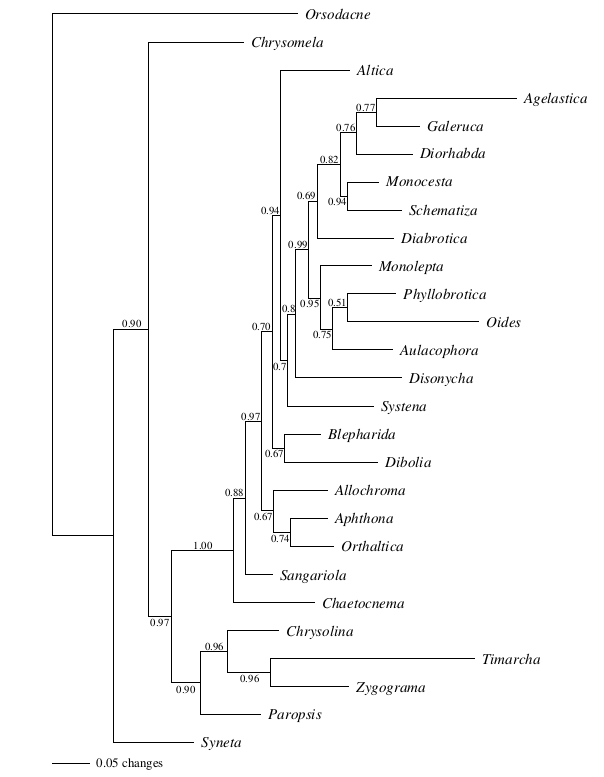
\includegraphics[height=5in]{fig8}
\caption{\textbf{\textsc{Bayesian phylogenetic tree of leaf beetles}}.
A majority rule tree of the trees sampled during the course of the MCMC analysis. The numbers at the interior nodes are the marginal posterior 
probability of the clade being correct.}
\label{fig8}
\end{figure}
The tree has additional information on it. For one, the numbers at the interior nodes represent the posterior probability of that clade being
correct (again, assuming the model is correct). For another, the branch lengths on the majority rule tree are proportional to the mean 
of the posterior probability of the branch length. 

The Bayesian analysis also provided information on the parameters of the model. Appendix 3
summarizes the marginal posterior probability of each parameter. There are a few points to note here. First, the nonsynonymous/synonymous
rate ratio ($\omega$) is estimated to be a very small number. This is consistent with the EF-1$\alpha$ gene being under strong purifying
selection. Second, the rate multiplier parameters for the site specific model ($m_1, m_2, m_3, m_4$) indicate that the rate of substitution
is different for the gene regions. The stem partition of the ribosomal gene is the most conservative. Third, the doublet stationary frequency
parameters ($\pi_{AA} \ldots \pi_{TT}$) are consistent with a pattern of higher rates to Watson-Crick doublets; note that the stationary
frequency is highest for the AT, TA, GC, and CG doublets. Finally, in this analysis we allowed the stationary frequencies of the states
to be random variables, and integrated over uncertainty in them. All of the state frequency parameters were given a flat Dirichlet prior. Although the
base frequencies are commonly estimated via maximum likelihood for simple ($4 \times 4$) models, they are rarely estimated for codon models.
Instead, they are usually estimated by using the observed frequencies of the nucleotides at the three codon positions to predict the
codon frequencies. In the Bayesian analysis, on the other hand, estimating these parameters is not too onerous.

The only parameter not shown in Appendix 3 is the amino acid model, which was treated as unknown in this analysis. The Markov chain
proposed moves among 10 different amino acid models (the ones listed earlier). The chain visited the Mtrev model almost all of the time, giving
it a posterior probability of 1.0. The results of the Bayesian analysis confirm our guess that the Mtrev should be the most reasonable of the amino acid models, because
it was estimated using a data base of mitochondrial sequences. Importantly, we did not need to rely on our guess of what amino acid
model to use, and could let the data inform us about the fit of the alternative models.

\subsection{Estimating divergence times}

The molecular clock hypothesis states that substitutions accumulate at roughly the same rate along different lineages of a phylogenetic tree ([REF]). 
Besides being among the earliest ideas in molecular evolution, the molecular clock hypothesis is an immensely useful one. If true, it suggests
a way to estimate the divergence times of species with poor fossil records. The idea, in its simplest form, is shown in Figure~9. The figure shows
a tree of three species. The numbers on the branches are the branch lengths, in terms of expected number of substitutions per site.
Note that the branch lengths on the tree satisfy the molecular clock hypothesis; if you sum the lengths of the branches from the root to each of the
tips, you get the same number (0.4). One can estimate branch lengths under the molecular clock hypothesis by constraining the branch lengths to have
this property. Figure~9 shows the second key assumption that must be made to estimate divergence times. We assume that the divergence of at least
one of the clades on the tree is known. In this hypothetical example, we assume that species A and B diverged five million years ago. We have calibrated
the molecular clock. The calibration is this: if five million years have elapsed since the common ancestor of A and B, then 0.1 substitutions is equal
to five million years. Together, the assumptions of a molecular clock and a calibration allow us to infer that the ancestor of the three species must have
diverged 20 million years ago.
\begin{figure}[t]
\centering
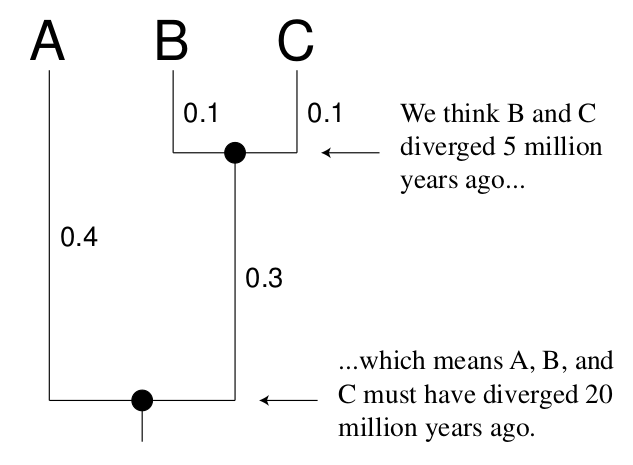
\includegraphics[height=2in]{fig9}
\caption{\textbf{\textsc{Estimating divergence times using the molecular clock}}.
A tree of three species showing how divergence times can be estimated.}
\label{fig9}
\end{figure}

There are numerous potential problems with the simple picture we presented. We will list them here:
\begin{itemize}
\item Substitutions may not accumulate at the same rate along different lineages. In fact, it is easy to test the molecular clock hypothesis, using
for example a likelihood ratio test (Felsentein, 1981). The molecular clock hypothesis is usually rejected for real data sets. 

\item Even if the molecular clock is true, we do not know the lengths of the branches with certainty. In fact, there are potential errors not
only in the branch lengths but also in the tree.

\item We do not know the divergence times of any of the species on the tree with absolute certainty. This uncertainty should in some way be accommodated.
\end{itemize}
The first problem---that substitutions may not accumulate at a constant rate along the phylogenetic tree---has received the most attention from biologists. 
Many statistical tests have been devised to examine whether rates really are constant over the tree. As already mentioned, applying these tests to
real data usually results in the molecular clock being rejected. However, it is still possible that divergence times can be estimated even if the clock
is not perfect. Perhaps the tests of the molecular clock are sensitive enough to pick up on small amounts of rate variation, but that the degree of rate variation
does not scupper our ability to estimate divergence times.
Some biologists have attempted to account for the variation in rates. One approach is to find taxa that are the worst offenders of the clock and either eliminate
them, or allow a different rate just for those taxa. Another approach specifies a parametric model describing how substitution rates change on the tree. These
relaxed clock models still allow estimation of divergence times, but may correct for limited degrees of rate variation across lineages. To date, two different
models have been proposed for allowing rates to vary across the tree ([REFS]), and in both cases, a Bayesian MCMC approach was taken to estimate parameters.

In the remainder of this section, we will assume that the molecular clock is true, or at least that if the molecular clock is violated, we can still meaningfully estimate divergence
times. The point of this section is not to provide a definitive answer to the divergence time of any particular group, but rather to show how uncertainty in the tree, 
branch lengths, and calibration times can be accounted for in a Bayesian analysis. We examine two data sets. The first 
data set included complete
mitochondrial protein-coding sequences from 23 mammals ({\sc Arnason} {\it et al}.\ 1997). We excluded the platypus ({\it Ornithorhynchus anatinus}) and the
guinea pig ({\it Cavia porcellus}) from our analysis. We analyzed the alignment of mitochondrial sequences under the GTR+SS model of DNA substitution. The
data were partitioned by codon position, and the rates for first, second, and third positions estimated. The second data set consists of 104 amino acid sequences sampled from
mouse, rate, an artiodactyl, human, and chicken
collated by Nei et al. (2001). Nei et al. (2001) were mainly interested in estimating the divergence times of the rodents and the rodent-human split, and pointed out the
importance of taking a multi-gene approach to divergence time estimation. We analyze their data using the partitioned approach, described in the previous section. We
partition the data by gene, resulting in 104 divisions in the data. We allow rates to vary systematically across genes using the site specific model. We allow rates to
vary within genes by treating the rate of substitution at an amino acid position as a gamma-distributed random variable. We allow different gamma shape parameters
for each partition. Moreover, we allow a different amino acid model for each partition, with the actual identity of the amino acid model being unknown.
For both data sets, we constrained the branch lengths to obey the molecular clock hypothesis. MrBayes was used to approximate the joint posterior probability of
all of the parameters of the evolutionary model. For the mammalian mitochondrial alignment, we ran the MCMC algorithm for a total of one million cycles and based
inferences on samples taken during the last 900,000 MCMC cycles. For the amino acid alignments, we ran two independent Markov chains, each for a total of three
million update cycles. We combined the samples taken after the 500,000th cycle.

For the mammalian data set, we had a total of 9,000 trees with branch lengths that were sampled from the posterior probability distribution of trees. Each of the trees obeyed
the molecular clock, meaning that the if one were to take a direct path from each tip of the tree to the root, and sum the lengths of the branches on each path, one would
obtain the same number. Importantly, the lengths of the branches and the topology of the tree differed from one sample to another. The differences reflect the uncertainty
in the data about the tree and branch lengths. The final missing ingredient is a calibration time for some divergence time on the tree. We used the divergence between
the cow and the whales as the calibration. Our first analysis of these samples will reflect the typical approach taken when estimating divergence times; we will assume
that the divergence between cows and whales was {\it precisely} 56.5 million years ago. This is a reasonable guess at the divergence time of cows and whales. Figure~10
shows the posterior probability distribution of the divergence time at the root of the tree, corresponding to the divergence of marsupial and placental mammals. 
\begin{figure}[t]
\centering
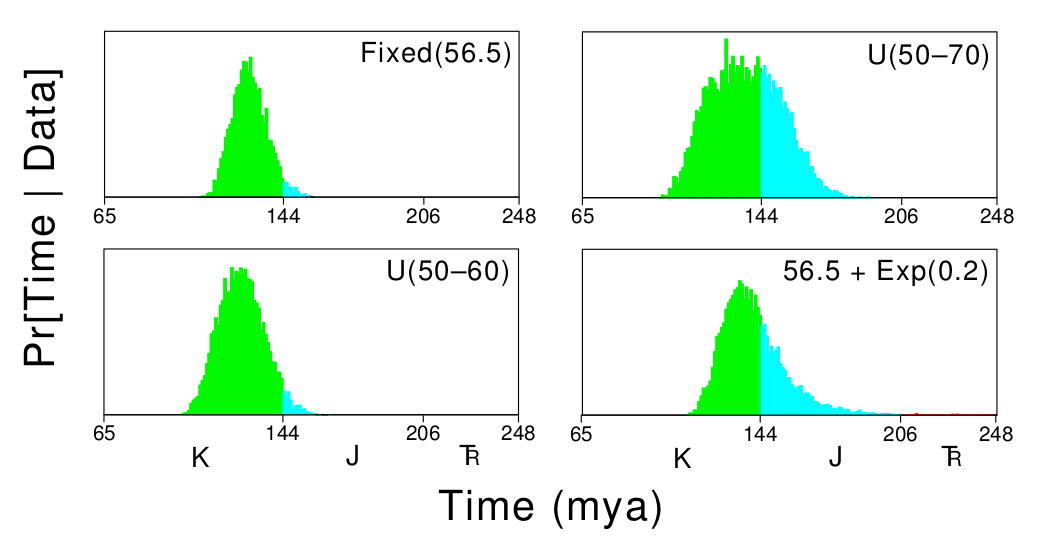
\includegraphics[height=2.3in]{fig10}
\caption{\textbf{\textsc{The posterior probability density distribution of the divergence time of placental and marsupial mammals}}.
The distributions were calculated assuming the divergence time between cows and whales was precisely 56.5 million years [Fixed(56.5)], uniformly
distributed between two times (U) or no less than 56.5 million years, with an exponentially declining prior into the past [56.5 + Exp(0.2)]. K, J, and Tr are the Cretaceous,
Jurassic, and Triassic time periods, respectively.}
\label{fig10}
\end{figure}
The top-left panel, marked `Fixed(56.5)' shows the posterior probability of the marsupial-placental split when the cow and whales are assumed to diverge precisely 56.5 million
years ago. It shows that even when we assume that the molecular clock is true and the calibration time is known without error, that there is considerable uncertainty about
the divergence time. The 95\% credible interval for the divergence of marsupials from placentals is (115.6, 145.1), a span of about 30 million years in the early Cretaceous.
In fact, it is easy to calculate the probability that the divergence time was in any specific time interval; with (posterior) probabilities 0.0, 0.97, 0.03, and 0.0, the divergence was
in the late Cretaceous, early Cretaceous, late Jurassic, and middle Jurassic, respectively. These probabilities account for the uncertainty in the topology of the tree, branch lengths
on the tree, and parameters of the substitution model, but do assume that the calibration time was perfectly known.

The other three panels in Figure~10 show the posterior probability distribution of the divergence of marsupial and placental mammals when the calibration is not assumed
known with certainty. In two of the analyses, we assumed that the cow and whales diverged at some unknown time, constrained to lie in an interval. The probability of
the divergence at any time in the interval was uniformly distributed. The last analysis, shown in the lower-right panel of Figure~10, assumed that the divergence of cows
and whales occurred no more recently than 56.5 million years, and was exponentially distributed before then (an offset exponential prior). As expected, the effect of introducing
uncertainty in the calibration times is reflected in a posterior probability distribution that is more spread out. The additional uncertainty can be neatly summarized by
the 95\% credible intervals:
\begin{center}
\begin{tabular}{lcc}
Prior & Credible Interval &Size \\ \hline
Fixed(56.5) & (115.6, 145.1) & 29.5\\
U(50, 60) & (107.8, 145.8) & 38.0 \\
U(50, 70) & (110.3, 166.9) & 56.6\\
56.5 + Exp(0.2) & (119.8, 175.6) & 55.8\\ 
\end{tabular}
\end{center}
The column marked `Size' shows the duration of the credible interval in millions of years. Clearly, introducing uncertainty in the calibration time is reflected in the posterior probability
distribution; and the credible interval becomes larger as more uncertainty is introduced into the calibration time.

\begin{figure}[t]
\centering
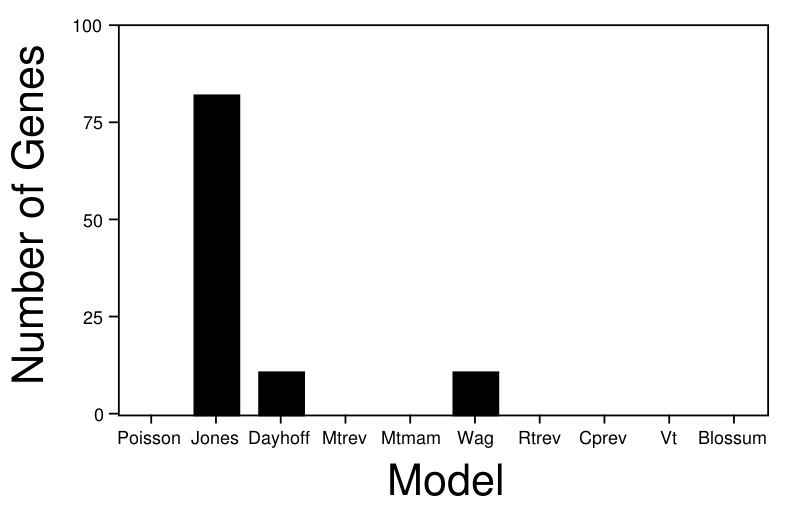
\includegraphics[height=2.3in]{fig11}
\caption{\textbf{\textsc{The distribution of best amino acid models for the 104 amino acid alignments}}.
The number of alignments  for which each amino acid model was best for the Nei et al. (2001) study.}
\label{fig11}
\end{figure}
The results from the analysis of the 104 concatenated amino acid alignments was similar to that of the mammalian mitochondrial data. However, the model for the amino acid
data sets was quite complicated. Besides the tree and branch lengths, there were 104 gamma shape parameters, 104 rate multipliers for the site specific model, and 104 unknown
amino acid models to estimate. We do not attempt to summarize the information for all of these parameters here. We only show the results for the amino acid models. Figure~11
shows which models were chosen as best for the various amino acid alignments. in 82 cases, the model of Jones et al. (1992) was chosen as best. The Dayhoff and Wag models
(Dayhoff et al., 1978; Whelan and Goldman, 2001) were chosen 11 times each. The other seven amino acid models were never chosen as the best one in any of the
104 alignments, though some did receive considerable posterior probability. There was no uncertainty in the topology of the tree chosen using the Bayesian method (Figure~12).

\begin{figure}[b]
\centering
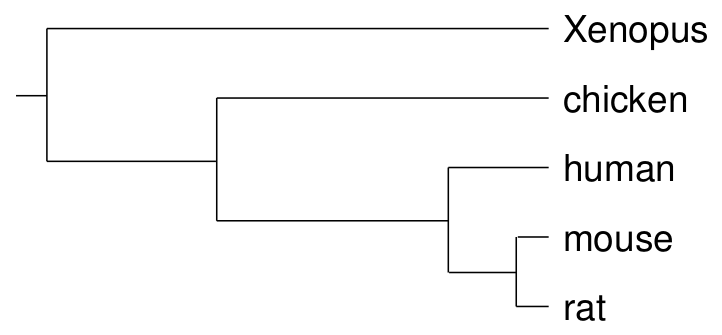
\includegraphics[height=1.5in]{fig12}
\caption{\textbf{\textsc{The best tree for the 104 amino acid alignments}}.
This tree had a posterior probability approximated to be 1.0 by the MCMC algorithm. The lengths of the branches are the mean of the posterior
probability distribution.}
\label{fig12}
\end{figure}
Nei et al. (2001) assumed as the calibration time the divergence of birds and mammals, which they assumed occurred 310 million years ago. Table~4 summarizes the results
of the divergence times for three clades on the tree, assuming the calibration time of Nei et al. (2001) as well as three other calibrations which allow for uncertainty in the
divergence time of birds and mammals.
\begin{table}[t]
\centering
\caption{\textbf{\textsc{Credible intervals for divergence times of the amino acid data}}.
The 95\% credible intervals for the divergence of mouse from rat, human from rodents, and the time at
the root of the tree for four different calibrations of the bird-mammal split.}
\begin{tabular}{l c c c} \hline
Calibration & Mouse-Rat & Human-Rodent & Root \\ \hline
310 & (25.9, 33.4) & (84.5, 97.5) & (448.3, 487.8) \\
U(288, 310) & (25.0, 33.0) & (80.6, 97.5) & (427.7, 491.8) \\
288 + Exp(0.1) & (24.6, 32.6) & (79.8, 96.6) & (423.3, 495.1) \\
288 + Exp(0.05) & (24.9, 34.9) & (80.4, 106.5) & (426.4, 551.6) \\ 
\hline
\end{tabular}
\label{tab4}
\end{table}
As might be expected, the uncertainty is greater for the older divergences. Also, having a calibration time that is older than the group
of interest makes the posterior probability distribution less vulnerable to errors in the calibration time.

The prior models for the uncertainty in the calibration times we used here are largely arbitrary, and chosen mostly to make the point that
errors in calibration times can be accounted for in a Bayesian analysis and that these errors can make a difference in the results (at least, these errors can
make a difference in how much one believes the results). Experts in the fossils from these groups would place very different priors on
the calibration times. For example Philip Gingerich (pers. comm.) would place a much smaller error on the divergence times between
cow and whales than we did here; the fossil record for this group is rich, and it is unlikely that cows and whales diverged as early as 100 million
years ago (our offset exponential prior places some weight on this hypothesis, along with divergences that are much earlier).
Lee (1999) pointed out that the widely used bird-mammal calibration of 310 million years is poorly chosen. The earliest synapsids (fossils
on the lineage leading to modern day mammals) is from the upper Pennsylvanian, about 288 million years ago. This is much more recent than
the calibration of 310 million years used by some to calibrate the molecular clock. 

\section{Conclusions}
\label{sec:4}

[To be completed.]


\section{References}

\newpage

\section*{Appendix 1}

{\bf All possible time-reversible models of DNA substitution}

\begin{center}
\begin{tabular}{cccccc} \hline
  $M_{1} = 111111$ &  $M_{35} = 122322$ &  $M_{69} = 121322$ & $M_{103} = 112132$ & $M_{137} = 121314$ & $M_{171} = 112343$ \\
  $M_{2} = 122222$ &  $M_{36} = 122232$ &  $M_{70} = 121232$ & $M_{104} = 112123$ & $M_{138} = 121134$ & $M_{172} = 112334$ \\
  $M_{3} = 121111$ &  $M_{37} = 122223$ &  $M_{71} = 121223$ & $M_{105} = 111233$ & $M_{139} = 112341$ & $M_{173} = 112342$ \\
  $M_{4} = 112111$ &  $M_{38} = 123111$ &  $M_{72} = 122312$ & $M_{106} = 111232$ & $M_{140} = 112314$ & $M_{174} = 112324$ \\
  $M_{5} = 111211$ &  $M_{39} = 121311$ &  $M_{73} = 122321$ & $M_{107} = 111223$ & $M_{141} = 112134$ & $M_{175} = 112234$ \\
  $M_{6} = 111121$ &  $M_{40} = 121131$ &  $M_{74} = 122132$ & $M_{108} = 112233$ & $M_{142} = 111234$ & $M_{176} = 123412$ \\
  $M_{7} = 111112$ &  $M_{41} = 121113$ &  $M_{75} = 122123$ & $M_{109} = 112323$ & $M_{143} = 123344$ & $M_{177} = 123421$ \\
  $M_{8} = 112222$ &  $M_{42} = 112311$ &  $M_{76} = 122231$ & $M_{110} = 112332$ & $M_{144} = 123434$ & $M_{178} = 123142$ \\
  $M_{9} = 121222$ &  $M_{43} = 112131$ &  $M_{77} = 122213$ & $M_{111} = 121233$ & $M_{145} = 123443$ & $M_{179} = 123124$ \\
 $M_{10} = 122122$ &  $M_{44} = 112113$ &  $M_{78} = 123311$ & $M_{112} = 121323$ & $M_{146} = 123244$ & $M_{180} = 123241$ \\
 $M_{11} = 122212$ &  $M_{45} = 111231$ &  $M_{79} = 123131$ & $M_{113} = 121332$ & $M_{147} = 123424$ & $M_{181} = 123214$ \\
 $M_{12} = 122221$ &  $M_{46} = 111213$ &  $M_{80} = 123113$ & $M_{114} = 122133$ & $M_{148} = 123442$ & $M_{182} = 121342$ \\
 $M_{13} = 122111$ &  $M_{47} = 111123$ &  $M_{81} = 121331$ & $M_{115} = 122313$ & $M_{149} = 122344$ & $M_{183} = 121324$ \\
 $M_{14} = 121211$ &  $M_{48} = 122333$ &  $M_{82} = 121313$ & $M_{116} = 122331$ & $M_{150} = 122343$ & $M_{184} = 121234$ \\
 $M_{15} = 121121$ &  $M_{49} = 123233$ &  $M_{83} = 121133$ & $M_{117} = 123123$ & $M_{151} = 122334$ & $M_{185} = 122341$ \\
 $M_{16} = 121112$ &  $M_{50} = 123323$ &  $M_{84} = 123211$ & $M_{118} = 123132$ & $M_{152} = 123423$ & $M_{186} = 122314$ \\
 $M_{17} = 112211$ &  $M_{51} = 123332$ &  $M_{85} = 123121$ & $M_{119} = 123213$ & $M_{153} = 123432$ & $M_{187} = 122134$ \\
 $M_{18} = 112121$ &  $M_{52} = 123322$ &  $M_{86} = 123112$ & $M_{120} = 123231$ & $M_{154} = 123243$ & $M_{188} = 123455$ \\
 $M_{19} = 112112$ &  $M_{53} = 123232$ &  $M_{87} = 122311$ & $M_{121} = 123312$ & $M_{155} = 123234$ & $M_{189} = 123454$ \\
 $M_{20} = 111221$ &  $M_{54} = 123223$ &  $M_{88} = 122131$ & $M_{122} = 123321$ & $M_{156} = 123342$ & $M_{190} = 123445$ \\
 $M_{21} = 111212$ &  $M_{55} = 122332$ &  $M_{89} = 122113$ & $M_{123} = 123444$ & $M_{157} = 123324$ & $M_{191} = 123453$ \\
 $M_{22} = 111122$ &  $M_{56} = 122323$ &  $M_{90} = 121321$ & $M_{124} = 123433$ & $M_{158} = 123144$ & $M_{192} = 123435$ \\
 $M_{23} = 111222$ &  $M_{57} = 122233$ &  $M_{91} = 121312$ & $M_{125} = 123343$ & $M_{159} = 123414$ & $M_{193} = 123345$ \\
 $M_{24} = 112122$ &  $M_{58} = 121333$ &  $M_{92} = 121231$ & $M_{126} = 123334$ & $M_{160} = 123441$ & $M_{194} = 123452$ \\
 $M_{25} = 112212$ &  $M_{59} = 123133$ &  $M_{93} = 121213$ & $M_{127} = 123422$ & $M_{161} = 121344$ & $M_{195} = 123425$ \\
 $M_{26} = 112221$ &  $M_{60} = 123313$ &  $M_{94} = 121132$ & $M_{128} = 123242$ & $M_{162} = 121343$ & $M_{196} = 123245$ \\
 $M_{27} = 121122$ &  $M_{61} = 123331$ &  $M_{95} = 121123$ & $M_{129} = 123224$ & $M_{163} = 121334$ & $M_{197} = 122345$ \\
 $M_{28} = 121212$ &  $M_{62} = 112333$ &  $M_{96} = 112331$ & $M_{130} = 122342$ & $M_{164} = 123413$ & $M_{198} = 123451$ \\
 $M_{29} = 121221$ &  $M_{63} = 112322$ &  $M_{97} = 112313$ & $M_{131} = 122324$ & $M_{165} = 123431$ & $M_{199} = 123415$ \\
 $M_{30} = 122112$ &  $M_{64} = 112232$ &  $M_{98} = 112133$ & $M_{132} = 122234$ & $M_{166} = 123143$ & $M_{200} = 123145$ \\
 $M_{31} = 122121$ &  $M_{65} = 112223$ &  $M_{99} = 112321$ & $M_{133} = 123411$ & $M_{167} = 123134$ & $M_{201} = 121345$ \\
 $M_{32} = 122211$ &  $M_{66} = 123122$ & $M_{100} = 112312$ & $M_{134} = 123141$ & $M_{168} = 123341$ & $M_{202} = 112345$ \\
 $M_{33} = 123333$ &  $M_{67} = 123212$ & $M_{101} = 112231$ & $M_{135} = 123114$ & $M_{169} = 123314$ & $M_{203} = 123456$ \\
 $M_{34} = 123222$ &  $M_{68} = 123221$ & $M_{102} = 112213$ & $M_{136} = 121341$ & $M_{170} = 112344$ &                    \\ \hline
\end{tabular}
\end{center}

\newpage

\section*{Appendix 2}

{\bf Using MrBayes 3.0.} MrBayes 3.0 (Huelsenbeck and Ronquist, 2001; Ronquist and Huelsenbeck, 2003) is a program distributed free
of charge and can be downloaded from the WWW at {\tt http://www.mrbayes.net}. The program takes as input an alignment of DNA,
RNA, amino acid, or restriction site site data (matrices of morphological characters can be input too). The program uses Markov chain
Monte Carlo to approximate the joint posterior probability distribution of the phylogenetic tree, branch lengths, and substitution model
parameters. The parameter values sampled by the Markov chain are saved to two files; one file contains the trees that were sampled
whereas the other file has the parameter values that were sampled. The program also provides some commands for summarizing the
results. The basic steps (and commands) that need to be executed to perform a Bayesian analysis of phylogeny using MrBayes include:
(1) reading in the data file (`execute [file name]'); (2) setting the model (using the `lset' and `prset' commands); (3) running the 
Markov chain Monte Carlo algorithm (using the `mcmc' command); and (4) summarizing the results (using the `sumt' and `sump' commands).
The program has extensive online help, which can be reached using the `help' command. We urge the user to explore the available commands
and the extensive amount we have written about each by exploring the `help' option.

\bigskip

\noindent {\bf Analyzing the `toy' example of simulated data.} The data matrix analyzed in numerous places in the text was simulated on the
tree of Figure~5 under the HKY85 model of DNA substitution. The specific HKY85 parameter values and the branch lengths used for the
simulation can be found in the text. The input file contained the alignment of sequences and the commands: 
 \begin{verbatim}
begin data;
   dimensions ntax=5 nchar=50;
   format datatype=dna;
   matrix
   Species_1   TAACTGTAAAGGACAACACTAGCAGGCCAGACGCACACGCACAGCGCACC 
   Species_2   TGACTTTAAAGGACGACCCTACCAGGGCGGACACAAACGGACAGCGCAGC 
   Species_3   CAAGTTTAGAAAACGGCACCAACACAACAGACGTATGCAACTGACGCACC 
   Species_4   CGAGTTCAGAAGACGGCACCAACACAGCGGACGTATGCAGACGACGCACC 
   Species_5   TGCCCTTAGGAGGCGGCACTAACACCGCGGACGAGTGCGGACAACGTACC 
   ;
end;

begin mrbayes;
   lset nst=2 rates=equal;
   mcmc ngen=1000000 nchains=1 samplefreq=100 printfreq=100;
   sumt burnin=1001;
   sump burnin=1001;
end;
\end{verbatim}
The actual alignment is in a NEXUS file format. More accurately, the input file format
is NEXUS(ish), because we do not implement all of the NEXUS standards in the program, and have
extended the format in some (unlawful) ways. The data are contained in the `data block' which starts
with a `begin data' command and ends with an `end' command. The next block is specific to
the program, and is called a `MrBayes'  block. Other programs will simply skip this block of commands,
just as MrBayes skips over foreign blocks it does not understand. All of the commands that can be issued
to the program via the command line can also be embedded directly into the file. This facilitates batch
processing of data sets. 

The first command sets the model to the HKY85 with no rate variation across sites. The second command runs
the MCMC algorithm, and the third and fourth commands summarize the results of the MCMC analysis, discarding
the first 1001 samples taken by the chain. Inferences, then, are based on the last 9,000 samples taken from the
posterior probability distribution.

\bigskip

\noindent {\bf Analyzing the leaf beetle data under a complicated model.} The following shows the data and MrBayes
block used in the analysis of the Kim et al. (2003) alignment of three different genes. We do not show the entire
alignment, though we do show the most relevant portions of the data block. Specifically, we show that you need to
specify the datatype as mixed when you perform a simultaneous Bayesian analysis on different types of data:
\begin{verbatim}
begin data;
   dimensions ntax=27 nchar=1090;
   format datatype=mixed(rna:1-516,dna:517-936,protein:937-1090) gap=- missing=?;
   matrix
   Orsodacne       gGGUAAACCUNAGaA [ 1060 other sites ] DPILYQHLFWFFGHP
   Chrysomela      GGGUAAACCUGAGAA [ 1060 other sites ] DPILYQHLFWFFGHP
   Altica          --------------- [ 1060 other sites ] DPILYQHLFWFFGHP
   Agelastica      GGGUAAACCUGAGAA [ 1060 other sites ] DPILYQHLFWFFGHP
   Monolepta       GGGUAAACCUGAGAA [ 1060 other sites ] DPILYQHLFWFFGHP
   Phyllobrotica   ---------UGANAA [ 1060 other sites ] DPILYQHLFWFFGHP
   Allochroma      GGGUAAaCcUGAgAA [ 1060 other sites ] DPILYQHLFWFFGHP
   Chrysolina      GGGUAAACCUGAGAA [ 1060 other sites ] DPILYQHLFWFFGHP
   Aphthona        GGGUAACCCUGAGAA [ 1060 other sites ] ???????????????
   Chaetocnema     --------------- [ 1060 other sites ] DPILYQHLFWFFGHP
   Systena         ---CCGACCUGAGAA [ 1060 other sites ] DPILYQHLFWFFGHP
   Monocesta       ----------GAGAA [ 1060 other sites ] DPILYQHLFWFFGHP
   Disonycha       -------------AA [ 1060 other sites ] DPILYQHLFWFFGHP
   Blepharida      --------------- [ 1060 other sites ] DPILYQHLFWFFGHP
   Galeruca        GGGUAAACCUGAGAA [ 1060 other sites ] DPILYQHLFWFFGHP
   Orthaltica      GGGUAAACCUGAGAA [ 1060 other sites ] DPILYQHLFWFFGHP
   Paropsis        GGGUAAACCUGAGAA [ 1060 other sites ] DPILYQHLFWFFGHP
   Timarcha        -----AACCUGAGAA [ 1060 other sites ] DPILYQHLFWFFGHP
   Zygograma       GGGUAAACCUGAGAA [ 1060 other sites ] DPILYQHLFWFFGHP
   Syneta          -----GAACUUACAA [ 1060 other sites ] DPILYQHLFWFFGHP
   Dibolia         ggguaaaccugagaa [ 1060 other sites ] DPILYQHLFWFFGHP
   Sangariola      --------------- [ 1060 other sites ] DPILYQHLFWFFGHP
   Aulacophora     -----------AGAA [ 1060 other sites ] DPILYQHLFWFFGHP
   Diabrotica      GGGUAAACcUGAgAA [ 1060 other sites ] DPILYQHLFWFFGHP
   Diorhabda       -----------AGAA [ 1060 other sites ] DPILYQHLFWFFGHP
   Schematiza      -----????UGAGAA [ 1060 other sites ] DPILYQHLFWFFGHP
   Oides           GGGUAACCCUGAGAA [ 1060 other sites ] DPILYQHLFWFFGHP
   ;
end;

begin mrbayes;
   pairs 22:497,  21:498,  20:499,  19:500,  18:501,  17:502,  16:503,  33:172, 
	         34:171,  35:170,  36:169,  37:168,  38:167,  45:160,  46:159,  47:158, 
	         48:157,  49:156,  50:155,  51:154,  53:153,  54:152,  55:151,  59:150, 
	         60:149,  61:148,  62:147,  63:146,  86:126,  87:125,  88:124,  89:123, 
	        187:484, 186:485, 185:486, 184:487, 183:488, 182:489, 191:295, 192:294, 
	        193:293, 194:292, 195:291, 196:290, 197:289, 198:288, 199:287, 200:286, 
	        201:283, 202:282, 203:281, 204:280, 205:279, 206:278, 213:268, 214:267, 
	        215:266, 216:265, 217:264, 226:259, 227:258, 228:257, 229:256, 230:255, 
	        231:254, 232:253, 233:252, 304:477, 305:476, 306:475, 307:474, 308:473, 
	        316:335, 317:334, 318:333, 319:332, 336:440, 337:439, 338:438, 339:437, 
	        340:436, 341:435, 343:422, 344:421, 345:420, 346:419, 347:418, 348:417, 
	        349:416, 351:414, 352:413, 353:412, 354:411, 355:408, 356:407, 357:406, 
	        358:405, 359:404, 360:403, 361:402, 369:400, 370:399, 371:398, 372:397, 
	        373:396, 376:394, 377:393, 379:392, 380:391, 381:390;
   charset ambiguously_aligned = 92-103 108-122 234-251 320-327 449-468;
   charset stems               =  22 497  21 498  20 499  19 500  18 501  17 502 
                                  16 503  33 172  34 171  35 170  36 169  37 168 
                                  38 167  45 160  46 159  47 158  48 157  49 156 
                                  50 155  51 154  53 153  54 152  55 151  59 150  
                                  60 149  61 148  62 147  63 146  86 126  87 125  
                                  88 124  89 123 187 484 186 485 185 486 184 487 
                                 183 488 182 489 191 295 192 294 193 293 194 292 
                                 195 291 196 290 197 289 198 288 199 287 200 286 
                                 201 283 202 282 203 281 204 280 205 279 206 278 
                                 213 268 214 267 215 266 216 265 217 264 226 259 
                                 227 258 228 257 229 256 230 255 231 254 232 253 
                                 233 252 304 477 305 476 306 475 307 474 308 473 
                                 316 335 317 334 318 333 319 332 336 440 337 439 
                                 338 438 339 437 340 436 341 435 343 422 344 421 
                                 345 420 346 419 347 418 348 417 349 416 351 414 
                                 352 413 353 412 354 411 355 408 356 407 357 406 
                                 358 405 359 404 360 403 361 402 369 400 370 399 
                                 371 398 372 397 373 396 376 394 377 393 379 392 
                                 380 391 381 390;
   charset loops               = 1-15 23-32 39-44 52 56-58 64-85 90-122 127-145 
                                 161-166 173-181 188-190 207-212 218-225 234-251 
                                 260-263 269-277 284 285 296-303 309-315 320-331 
                                 342 350 362-368 374 375 378 382-389 395 401 409 
                                 410 415 423-434 441-472 478-483 490-496 504-516;
   charset rna                 = 1-516;
   charset dna                 = 517-936;
   charset protein             = 937-1090;
   charset D2                  = 1-516;
   charset EF1a                = 517-936;
   charset EF1a1st             = 517-936\3;
   charset EF1a2nd             = 518-936\3;
   charset EF1a3rd             = 519-936\3;
   charset CO1aa               = 937-1090;
   partition by_gene_and_pos    = 5:rna,EF1a1st,EF1a2nd,EF1a3rd,CO1aa;
   partition by_gene            = 3:rna,EF1a,CO1aa;
   partition by_gene_and_struct = 4:stems,loops,EF1a,CO1aa;
   exclude ambiguously_aligned;
   set partition = by_gene_and_struct;
   lset applyto=(1) nucmodel=doublet;
   lset applyto=(2) nucmodel=4by4;
   lset applyto=(3) nucmodel=codon;
   lset applyto=(1,2,4) rates=gamma;
   lset nst=6;
   prset ratepr=variable aamodelpr=mixed;
   unlink shape=(all) revmat=(all);
   mcmc ngen=3000000 nchains=1 samplefreq=100 printfreq=100;
   sumt burnin=10001;
   sump burni=10001;
end;
\end{verbatim}
The commands in the MrBayes block show how to specify a very complicated model. 
First, we specify which nucleotides pair with one
another using the pairs command. We then specify a number of character sets, 
using the `charset' command. Specifying character
sets saves the hassle of having to type in a long list of character number 
every time you want to refer to some division of the data (such as
a gene). We then specify three character partitions. A character 
partition divides the data into groups of characters. Each character in
the matrix must be assigned to one, and only one, group. For example, 
one of the partitions we define (by\_gene) divides  the characters
into three groups. When a data file is executed it sets up a default partition of the data, that groups characters by data type. We need to tell
the program which of the four partitions to use (where the four partitions are default, by\_gene\_and\_pos, by\_gene, and by\_gene\_and\_struct). We
do this using the set command. Finally, we use lset and prset to specify different models to different groups of characters. In fact, with the applyto option
in lset and prset and the link and unlink commands, one can specify a very large number of possible models that currently cannot be implemented with
any other phylogeny program. The last three commands in run the MCMC algorithm and then summarize the results.

\bigskip

\noindent {\bf Analyzing the 104 amino acid alignments.} The analysis of the data collated by Nei et al. (2001) was conceptually simple, though
laborious, to set up. The data block, as usual, has the alignment, this time in interleaved format. The MrBayes block has 104 character set definitions, 
specifies a partition, grouping positions by gene, sets the partition, and then sets up a model in which the parameters are estimated independently for
each gene and that enforces the molecular clock.
\begin{verbatim}
begin data;
   dimensions ntax=5 nchar=48092;
   format datatype=protein interleave=yes;
   matrix
   [The data for the 104 alignments was here. We do not
    include it here for obvious reasone (see the nchar
    command, above).]
   ;
end;

begin mrbayes;
   charset M00007  =     1 -   112;
   charset M00008  =   113 -   218;
   charset M00037  =   219 -   671;
   [There were another 98 character set definitions
    which we have deleted here.]
   charset N01447  = 45917 - 46694;
   charset N01456  = 46695 - 47285;
   charset N01479  = 47286 - 48092;
   partition by_gene = 104:M00007,M00008,M00037,[98 other partitions],N01447,N01456,N01479;
   set autoclose=yes nowarn=yes;
   set partition=by_gene;
   outgroup xenopus;
   lset rates=gamma;
   prset ratepr=variable aamodel=mixed brlenspr=clock:uniform;
   unlink shape=(all) aamodel=(all);
   mcmcp ngen=30000000 nchains=1 samplefreq=1000 savebrlens=yes;
end;
\end{verbatim}


\newpage

\section*{Appendix 3}

{\bf Parameter estimates for the leaf beetle data.} The numbers are the mean and 95\% credible interval of the posterior probability
density distribution for each parameter.

\begin{center}
\begin{tabular}{lc lc lc}
Param. & Mean (CI) & Param. & Mean (CI) & Param. & Mean (CI) \\ \hline
$V$            & 3.495 (3.209, 3.828) & $\pi_{G}$      & 0.222 (0.180, 0.267) & $\pi_{GAC}$    & 0.012 (0.008, 0.016) \\
$r_{CT}^{(1)}$ & 0.428 (0.187, 0.850) & $\pi_{T}$      & 0.285 (0.240, 0.332) & $\pi_{GAG}$    & 0.007 (0.006, 0.009) \\
$r_{CG}^{(1)}$ & 0.616 (0.166, 1.616) & $\pi_{AAA}$    & 0.023 (0.020, 0.024) & $\pi_{GAT}$    & 0.018 (0.016, 0.019) \\
$r_{AT}^{(1)}$ & 2.130 (0.703, 5.436) & $\pi_{AAC}$    & 0.006 (0.006, 0.008) & $\pi_{GCA}$    & 0.014 (0.012, 0.018) \\
$r_{AG}^{(1)}$ & 0.780 (0.340, 1.594) & $\pi_{AAG}$    & 0.019 (0.014, 0.023) & $\pi_{GCC}$    & 0.023 (0.019, 0.027) \\
$r_{AC}^{(1)}$ & 0.828 (0.214, 2.240) & $\pi_{AAT}$    & 0.005 (0.004, 0.006) & $\pi_{GCG}$    & 0.005 (0.005, 0.005) \\
$r_{CT}^{(2)}$ & 3.200 (2.037, 4.915) & $\pi_{ACA}$    & 0.011 (0.007, 0.013) & $\pi_{GCT}$    & 0.036 (0.034, 0.037) \\
$r_{CG}^{(2)}$ & 0.335 (0.116, 0.683) & $\pi_{ACC}$    & 0.021 (0.017, 0.024) & $\pi_{GGA}$    & 0.019 (0.014, 0.022) \\
$r_{AT}^{(2)}$ & 0.994 (0.522, 1.699) & $\pi_{ACG}$    & 0.006 (0.004, 0.009) & $\pi_{GGC}$    & 0.013 (0.006, 0.015) \\
$r_{AG}^{(2)}$ & 2.805 (1.702, 4.447) & $\pi_{ACT}$    & 0.025 (0.019, 0.027) & $\pi_{GGG}$    & 0.004 (0.004, 0.006) \\
$r_{AC}^{(2)}$ & 1.051 (0.541, 1.880) & $\pi_{AGA}$    & 0.020 (0.013, 0.021) & $\pi_{GGT}$    & 0.018 (0.015, 0.019) \\
$r_{CT}^{(3)}$ & 2.292 (1.471, 3.555) & $\pi_{AGC}$    & 0.016 (0.014, 0.019) & $\pi_{GTA}$    & 0.022 (0.017, 0.028) \\
$r_{CG}^{(3)}$ & 1.021 (0.400, 2.127) & $\pi_{AGG}$    & 0.004 (0.001, 0.007) & $\pi_{GTC}$    & 0.014 (0.008, 0.014) \\
$r_{AT}^{(3)}$ & 1.320 (0.766, 2.184) & $\pi_{AGT}$    & 0.001 (0.001, 0.002) & $\pi_{GTG}$    & 0.014 (0.012, 0.016) \\
$r_{AG}^{(3)}$ & 2.276 (1.424, 3.621) & $\pi_{ATA}$    & 0.003 (0.003, 0.004) & $\pi_{GTT}$    & 0.020 (0.016, 0.020) \\
$r_{AC}^{(3)}$ & 1.041 (0.575, 1.756) & $\pi_{ATC}$    & 0.025 (0.024, 0.029) & $\pi_{TAC}$    & 0.033 (0.030, 0.034) \\
$\omega$       & 0.010 (0.010, 0.012) & $\pi_{ATG}$    & 0.014 (0.009, 0.017) & $\pi_{TAT}$    & 0.011 (0.010, 0.016) \\
$\pi_{AA}$     & 0.001 (0.000, 0.004) & $\pi_{ATT}$    & 0.026 (0.016, 0.029) & $\pi_{TCA}$    & 0.020 (0.017, 0.026) \\
$\pi_{AC}$     & 0.004 (0.000, 0.008) & $\pi_{CAA}$    & 0.015 (0.011, 0.019) & $\pi_{TCC}$    & 0.026 (0.023, 0.033) \\
$\pi_{AG}$     & 0.006 (0.003, 0.012) & $\pi_{CAC}$    & 0.010 (0.009, 0.014) & $\pi_{TCG}$    & 0.015 (0.014, 0.016) \\
$\pi_{AT}$     & 0.122 (0.086, 0.170) & $\pi_{CAG}$    & 0.009 (0.006, 0.011) & $\pi_{TCT}$    & 0.025 (0.024, 0.037) \\
$\pi_{CA}$     & 0.003 (0.000, 0.008) & $\pi_{CAT}$    & 0.009 (0.005, 0.010) & $\pi_{TGC}$    & 0.003 (0.003, 0.005) \\
$\pi_{CC}$     & 0.005 (0.001, 0.013) & $\pi_{CCA}$    & 0.022 (0.021, 0.024) & $\pi_{TGG}$    & 0.014 (0.008, 0.016) \\
$\pi_{CG}$     & 0.257 (0.191, 0.319) & $\pi_{CCC}$    & 0.012 (0.011, 0.014) & $\pi_{TGT}$    & 0.001 (0.001, 0.003) \\
$\pi_{CT}$     & 0.002 (0.000, 0.005) & $\pi_{CCG}$    & 0.008 (0.003, 0.010) & $\pi_{TTA}$    & 0.020 (0.013, 0.025) \\
$\pi_{GA}$     & 0.001 (0.000, 0.003) & $\pi_{CCT}$    & 0.008 (0.007, 0.010) & $\pi_{TTC}$    & 0.045 (0.044, 0.049) \\
$\pi_{GC}$     & 0.284 (0.222, 0.353) & $\pi_{CGA}$    & 0.002 (0.001, 0.004) & $\pi_{TTG}$    & 0.025 (0.025, 0.026) \\
$\pi_{GG}$     & 0.003 (0.000, 0.008) & $\pi_{CGC}$    & 0.009 (0.009, 0.009) & $\pi_{TTT}$    & 0.011 (0.010, 0.011) \\
$\pi_{GT}$     & 0.078 (0.057, 0.106) & $\pi_{CGG}$    & 0.001 (0.000, 0.000) & $\alpha_1$     & 0.422 (0.308, 0.570) \\
$\pi_{TA}$     & 0.145 (0.103, 0.190) & $\pi_{CGT}$    & 0.016 (0.014, 0.016) & $\alpha_2$     & 0.381 (0.296, 0.484) \\
$\pi_{TC}$     & 0.004 (0.001, 0.008) & $\pi_{CTA}$    & 0.005 (0.004, 0.010) & $\alpha_4$     & 0.226 (0.175, 0.288) \\
$\pi_{TG}$     & 0.073 (0.056, 0.093) & $\pi_{CTC}$    & 0.016 (0.015, 0.020) & $m_1$          & 0.708 (0.553, 0.894) \\
$\pi_{TT}$     & 0.003 (0.001, 0.008) & $\pi_{CTG}$    & 0.042 (0.036, 0.046) & $m_2$          & 0.870 (0.732, 1.027) \\
$\pi_{A}$      & 0.252 (0.209, 0.301) & $\pi_{CTT}$    & 0.042 (0.034, 0.048) & $m_3$          & 1.274 (1.171, 1.378) \\
$\pi_{C}$      & 0.239 (0.199, 0.284) & $\pi_{GAA}$    & 0.034 (0.031, 0.044) & $m_4$          & 0.856 (0.651, 1.100) \\ \hline
\end{tabular}
\end{center}



\clearpage

\bibliographystyle{alpha}
\bibliography{bayes}
\printindex

\end{document}
